% !TeX program = pdflatex
% Orchestraton Economics — Business Draft v4
% Youssef Hariri, DeeWaanAI, 2026-08-08
\documentclass[12pt,a4paper]{article}

% ── Packages ──────────────────────────────────────────────────────
\usepackage[utf8]{inputenc}
\usepackage[T1]{fontenc}
\usepackage{lmodern}
\usepackage[margin=2.5cm]{geometry}
\usepackage{amsmath,amssymb}
\usepackage{graphicx}
\usepackage{booktabs}
\usepackage{longtable}
\usepackage{array}
\usepackage{multirow}
\usepackage{hyperref}
\usepackage{natbib}
\usepackage{caption}
\usepackage{subcaption}
\usepackage{enumitem}
\usepackage{xcolor}
\usepackage{mdframed}
\usepackage{csquotes}  % proper quotation marks
\usepackage{siunitx}
\usepackage{float}
\usepackage{tabularx}
\usepackage[capitalise,nameinlink]{cleveref}

% ── Custom commands ───────────────────────────────────────────────
\newcommand{\phiBlend}{\varphi}
\newcommand{\BF}{\ensuremath{\mathit{BF}}}
\newcommand{\TEGR}{\ensuremath{\text{T-EGR}}}
\newcommand{\dval}[1]{\ensuremath{d = #1}}
\newcommand{\CI}[1]{\ensuremath{#1}}
\newcommand{\figref}[1]{Figure~\ref{#1}}
\newcommand{\tabref}[1]{Table~\ref{#1}}
\newcommand{\secref}[1]{Section~\ref{#1}}

% ── Executive-summary box ─────────────────────────────────────────
\mdfdefinestyle{execsummary}{
  linecolor=black,
  linewidth=1.5pt,
  backgroundcolor=gray!5,
  innertopmargin=10pt,
  innerbottommargin=10pt,
  innerrightmargin=10pt,
  innerleftmargin=10pt,
  skipabove=\bigskipamount,
  skipbelow=\bigskipamount,
}

% ── Hyperref setup ────────────────────────────────────────────────
\hypersetup{
  colorlinks=true,
  linkcolor=blue!60!black,
  citecolor=green!40!black,
  urlcolor=blue!70!black,
}

% ── Title ─────────────────────────────────────────────────────────
\title{\textbf{Orchestrate or Upgrade? The Cost--Quality Economics of
Multi-Agent Pipelines versus Frontier Models --- When Lower Tier Teams
Deliver 98\% Quality at 23\% Cost}}

\author{Youssef Hariri\\
\small DeeWaanAI\quad $\cdot$\quad \texttt{osf.io/mjb8x}\quad $\cdot$\quad 2026-08-08}

\date{}

% ==================================================================
\begin{document}
\maketitle

\begin{abstract}
\noindent
Organizations deploying large language models (LLMs) for knowledge work face a
strategic choice: invest in higher-tier models or invest in multi-agent pipeline
structures that orchestrate cheaper models. We test this resource-allocation
tradeoff with a pre-registered $2 \times 2 \times 2$ factorial experiment across
five LLM families, 38 business-strategy problems, and 1{,}900
generation--judgment runs evaluated by a blinded three-judge panel. Our findings
yield a decision framework for AI investment. First, team structure delivers
higher marginal returns at the cheap tier than at the frontier tier
($d = -0.227$, $p = 0.015$): a cheap model with a three-step pipeline
approaches frontier quality at 23\% of the cost ($\TEGR = 6.15$). Second,
personas degrade output quality on average ($d = -0.691$), representing a
failed investment in stylistic differentiation. Third, a low-cost refinement
pass recovers 60--64\% of the frontier gap but never achieves paired
superiority --- a bounded-improvement result that constrains the substitution
thesis. Qualitative coding ($\kappa = 0.824$) reveals that orchestration buys
coverage (more structure, more length) while the frontier wins on density
(compressed insight, zero boilerplate). The Pareto frontier is stable across
price assumptions, yielding actionable contingency rules for budget-constrained
firms. We contribute the T-EGR efficiency metric, a mechanistic account of why
structure substitutes for tier only partially, and a practitioner decision
framework that maps budget tier and task type to optimal pipeline architecture.

\medskip
\noindent\textbf{Keywords:} LLM Orchestration, Multi-Agent Pipelines,
Cost--Performance Analysis, LLM-as-a-Judge, T-EGR, Pre-registration.
\end{abstract}

\bigskip

% ── Executive Summary ─────────────────────────────────────────────
\begin{mdframed}[style=execsummary]
\textbf{Executive Summary for Practitioners}

\medskip
\noindent\textbf{Decision context.} A firm that needs LLM-generated knowledge
work can either (a)~pay for a frontier model or (b)~orchestrate cheaper models
into a multi-step pipeline. Which dollar buys more quality?

\medskip
\noindent\textbf{Bottom line.} Across 1{,}900 runs, five model families, and 38
business problems: a cheap solo model in a three-step builder--critic--refiner
pipeline delivers \textbf{98\% of frontier quality at 23\% of the cost}.
Orchestrating a frontier model costs \textbf{3.5$\times$ more for negligible
gain}. A \$0.002 refinement pass recovers most of the remaining gap but never
beats the frontier.

\medskip
\noindent\textbf{Three rules for AI budget allocation:}
\begin{enumerate}[leftmargin=*,nosep]
  \item \textbf{Cheap tier + pipeline structure} $\to$ highest ROI
    ($\TEGR$~6.15). Best for coverage-sensitive tasks: timelines, matrices,
    quantified plans.
  \item \textbf{Frontier tier + solo} $\to$ best absolute quality per dollar
    when density matters (compressed insight, zero boilerplate).
  \item \textbf{Never add personas as a quality lever} --- they increase cost
    while degrading judged quality ($d = -0.691$).
\end{enumerate}

\medskip
\noindent\textbf{Caveat.} Cheap teams buy \emph{coverage} (more structure, more
length); frontier models win on \emph{density} (insight per paragraph). If the
task rewards concise strategic principles, the frontier is worth the premium.
If the task rewards completeness, the cheap pipeline is the better bet.
\end{mdframed}

% ── List of Abbreviations ─────────────────────────────────────────
\section*{List of Abbreviations}
\small
\begin{longtable}{@{}ll@{}}
\toprule
\textbf{Abbr} & \textbf{Definition} \\
\midrule
$\BF_{10}$        & Bayes factor in favor of $H_1$ over $H_0$ \\
C-S-N             & cheap solo, no persona \\
C-S-P             & cheap solo, persona \\
C-T-N             & cheap team, no persona \\
C-T-P             & cheap team, persona \\
F-S-N             & frontier solo, no persona \\
F-S-P             & frontier solo, persona \\
F-T-N             & frontier team, no persona \\
F-T-P             & frontier team, persona \\
EGR               & Efficiency Gain Ratio \\
FDR               & false discovery rate \\
FLOPs             & floating-point operations \\
FSN               & frontier solo, no persona (baseline) \\
ICER              & incremental cost--effectiveness ratio \\
IRR               & inter-rater reliability \\
JZS               & Jeffreys--Zellner--Siow (Bayes factor prior) \\
LLM               & large language model \\
LMM               & linear mixed model \\
LOO               & leave-one-out \\
OBF               & O'Brien--Fleming (spending function) \\
SESOI             & smallest effect size of interest \\
T-EGR             & Tiered Efficiency Gain Ratio \\
TOST              & two one-sided tests (equivalence) \\
\bottomrule
\end{longtable}
\normalsize

% ==================================================================
% 1  INTRODUCTION
% ==================================================================
\section{Introduction}\label{sec:intro}

The past two years have seen a rapid industrial shift from single-model
inference to the orchestration of multiple language-model calls: pipelines
chain builder, critic, and refiner agents into structured workflows; agent
teams assign social roles to each step; panels of judges aggregate verdicts
across models. The implicit claim is economic --- that \emph{structure can
substitute for model tier}. A practitioner who cannot afford a frontier model,
the argument runs, can reach comparable output quality by composing cheaper
models into an orchestrated system. If true, the claim reshapes how
organizations price, budget, and architect generative-AI products. If false,
orchestration is at best a marginal convenience and at worst a cost multiplier
that never reaches frontier quality.

Prior empirical work on generative AI is encouraging but silent on this
specific claim. Controlled productivity studies show that a single generative
assistant raises output quality and reduces task time \citep{NoyZhang2023,
BrynjolfssonLiRaymond2023}, yet they treat the model as a given, single-agent
capability. A field experiment with consultants documented a ``jagged
technological frontier'': large gains inside the model's capability boundary,
large losses outside it \citep{DellAcquaEtAl2023}. Neither study varies the
structure around the model. Multi-agent and ensemble work shows that sampling,
debate, and tree search can improve accuracy \citep{WangEtAl2023,
LiangEtAl2024, YaoEtAl2023}, but the gains are reported without cost-matched
comparison to a stronger single model. A nascent theory of test-time compute
predicts that, for fixed problem difficulty, more inference compute on a
smaller model can outperform less inference compute on a larger one
\citep{SnellEtAl2024}, but its predictions are in units of FLOPs, not dollars,
and only on verifiable tasks.

Three gaps follow. First, no factorial, cost-matched comparison of orchestrated
cheap models versus frontier solo exists on open-ended tasks. Second, no
mechanistic account explains \emph{why} orchestration succeeds or fails ---
whether it adds structural coverage or compressed insight. Third, no economic
metric is robust to the price-assumption choices that inevitably shape per-run
costing.

This paper addresses all three. We run a pre-registered $2 \times 2 \times 2$
(tier $\times$ structure $\times$ persona) factorial experiment over five model
families, 38 domain-stratified business problems, and 1{,}900
generation--judgment runs, measured by a blinded three-judge panel from
families disjoint from every generator. Cost is stored as tokens and re-priced
through a frozen price vector under three blended input/output ratios, so every
reported dollar is reproducible and re-priceable. A second study applies a
cheap, add-only refinement pass to the orchestrated outputs and codes the
qualitative differences between original, refined, and frontier answers,
testing the mechanistic prediction that orchestration buys coverage while the
frontier wins on density.

Five contributions follow:
\begin{enumerate}[leftmargin=*,nosep]
  \item \textbf{First cost-matched pre-registered factorial on orchestration
        economics.} Negative superiority results are reported as primary
        findings, not buried as null results.
  \item \textbf{The T-EGR metric} (novelty ratio $\div$ cost ratio) and a
        price-assumption-robust Pareto frontier.
  \item \textbf{A mechanistic account} from a mixed-methods Study~2 (pooled
        $\kappa = 0.824$): orchestration buys coverage, the frontier wins on
        density.
  \item \textbf{The refinement boundary}: a \$0.002 refinement pass reaches
        parity with the weakest frontier but never superiority.
  \item \textbf{Practitioner contingency rules} mapping cell to use-case to
        expected T-EGR.
\end{enumerate}

The paper proceeds as follows. \cref{sec:lit} reviews related literature.
\cref{sec:method} describes the pre-registered design, apparatus, and analysis,
including an AI-assisted research disclosure (\cref{sec:ai-disclosure}).
\cref{sec:results} presents the results of both studies. \cref{sec:discussion}
discusses theoretical and practical implications. \cref{sec:limitations}
acknowledges limitations. \cref{sec:future} outlines future directions.
\cref{sec:conclusion} concludes.

% ==================================================================
% 2  LITERATURE REVIEW
% ==================================================================
\section{Literature Review}\label{sec:lit}

This review synthesizes four streams of research: (i)~measured productivity
effects of generative AI, (ii)~multi-agent and ensemble generation methods,
(iii)~LLM-as-a-judge evaluation methodology, and (iv)~open-science methods for
economic measurement. We then integrate these streams with our own prior work on
personas and efficiency metrics to articulate the research gap that motivates
this study.

\subsection{Productivity effects of generative AI}

\subsubsection{Measured gains in knowledge work}

Three controlled studies establish that generative AI raises knowledge-work
productivity, but they also reveal that the gains are conditional and bounded.
\citet{NoyZhang2023} randomized 444 mid-level professionals to ChatGPT-assisted
and control arms on professional writing tasks: assistance reduced completion
time by 0.8 standard deviations and raised output quality by 0.4 standard
deviations, with the largest quality gains among initially lower-performing
workers --- a compression of the performance distribution.
\citet{BrynjolfssonLiRaymond2023} observed 5{,}179 customer-support agents
using a generative assistant in the field and found a 14\% average productivity
increase, concentrated among novice and low-skilled workers (+34\%), consistent
with the model diffusing behaviors of high-ability agents across the workforce.

A critical limitation unites these studies: both treat the model as a
\emph{given, single-agent capability}. The unit of analysis is one model call,
not an orchestrated system. The professional-writing and customer-support tasks
they study are also relatively closed-form: the desired output is
well-specified (a support response, a draft document), and quality can be
partially verified against ground truth. Open-ended strategic tasks --- the
domain of this paper --- have no verifiable correct answer, which changes both
the nature of the ``frontier'' and the applicability of the productivity gains
documented above.

\subsubsection{The jagged frontier and its boundary}

The boundary of these gains is the central caution. \citet{DellAcquaEtAl2023}
ran a field experiment with 758 consultants on realistic professional problems
and documented a ``jagged technological frontier'': inside the model's
capability boundary, consultants completed 12.2\% more tasks, 25.1\% faster,
with 40\% higher quality; outside it, consultants using the model were 19
percentage points less likely to produce correct solutions than controls. Two
productive behavioral strategies emerged (``centaurs'' dividing work at the
boundary, ``cyborgs'' interleaving with the model), but neither changed the
location of the boundary itself.

The jagged frontier concept is especially consequential for open-ended tasks.
In closed-form domains (arithmetic, code, support scripts), the boundary is
sharp: a solution is either correct or not. In open-ended business strategy,
the boundary is diffuse --- there is no single correct answer, only better or
worse responses. This diffuseness creates a fundamental ambiguity: when a cheap
model produces a plausible but suboptimal strategy, the user may not know they
are ``outside the frontier'' until the solution fails in deployment. The open
question this paper addresses is whether \emph{orchestration structure} can
shift the effective capability frontier for these open-ended tasks --- and at
what cost.

\subsection{Multi-agent systems, reasoning, and inference-time compute}

\subsubsection{From chain-of-thought to structured reasoning}

The modern reasoning literature begins with the observation that language models
solve complex problems better when they generate intermediate reasoning steps.
\citet{WeiEtAl2022} introduced chain-of-thought (CoT) prompting: appending
exemplars that show step-by-step reasoning before the final answer elicited
comparable reasoning in the model, dramatically improving performance on
arithmetic, commonsense, and symbolic reasoning tasks. The CoT paradigm
reframed language-model inference from single-shot generation to
\emph{structured multi-step deliberation} --- a conceptual shift that enabled
the orchestration methods reviewed below.

CoT's direct descendant in the accuracy--cost tradeoff space is
self-consistency. \citet{WangEtAl2023} showed that sampling a diversity of
reasoning paths from a single model and taking a majority vote over final
answers improves arithmetic, commonsense, and symbolic reasoning well beyond
CoT decoding alone. The result establishes the general principle that parallel
sampled calls can be converted into accuracy. Its direct corollary --- that
accuracy is bought at a multiplicative cost in calls and tokens --- is rarely
priced against the alternative of a single stronger model.

\subsubsection{Interactive deliberation: debate, tree search, and agent loops}

Moving beyond independent sampling, recent work has explored \emph{interactive}
structures in which model instances influence each other. \citet{LiangEtAl2024}
showed that multiple LLM instances proposing answers, critiquing each other's
responses, and refining their own over debate rounds improves factuality and
reasoning on arithmetic and knowledge benchmarks, encourages divergent
thinking, and reliably converges to shared answers. \citet{YaoEtAl2023} extended
the reasoning structure from linear chains to branching trees: Tree of Thoughts
treats each reasoning step as a node in a search graph, allowing the model to
explore multiple reasoning paths, backtrack from dead ends, and select the most
promising branch --- deliberate problem solving rather than single-path
generation.

These works demonstrate that structure (sampling, aggregation, critique loops,
tree search) adds quality beyond a single call. What they do not provide is a
cost-matched factorial comparison: prior multi-agent studies report quality
gains without measuring dollars, and without comparing orchestrated cheap models
against an un-orchestrated frontier model on identical problems. The
substitution claim --- that structure can stand in for model tier --- is
therefore assumed, not tested.

\subsubsection{The test-time compute hypothesis}

A nascent theoretical framework reframes the model-tier-versus-structure
tradeoff as an allocation problem. \citet{SnellEtAl2024} demonstrated that
scaling inference-time computation (more tokens, verifier-based search,
iterative refinement) can be more effective than scaling model parameters for
improving performance on reasoning benchmarks. Their compute-optimal curve
predicts that for any fixed problem difficulty, there exists an optimal
allocation between training compute (model size) and inference compute
(test-time search). Below that optimum, a smaller model with more inference
compute outperforms a larger model with less; above it, the larger model wins.

This framework is the closest theoretical grounding for the ``orchestration
economics'' claim, but it remains limited in three ways that motivate our study.
First, \citet{SnellEtAl2024} measure \emph{verifiable} reasoning tasks (math,
code) where a verifier can score intermediate steps; open-ended business
strategy has no verifier. Second, their test-time compute is
\emph{search-based} (sampling + scoring), whereas the multi-agent literature
uses \emph{structural} compute (builder--critic--refiner pipelines, debate
rounds) --- the two may have different cost--quality curves. Third, and most
fundamentally, their analysis is in units of FLOPs, not dollars: the
practitioner facing an API bill cannot spend FLOPs. A dollar-matched empirical
test is missing.

\subsubsection{Self-refinement and the limits of iterative improvement}

The final reasoning structure relevant to this study is self-refinement: a
model critiquing and revising its own output. \citet{ShinnEtAl2023} introduced
Reflexion, in which a language agent maintains a reflective memory of past
failures and uses verbal reinforcement learning to improve subsequent trials.
On coding and decision-making tasks, Reflexion outperformed single-shot
baselines and even standard CoT by learning from its own errors.

Self-refinement raises a hypothesis directly tested in our Study~2: if a cheap
model's initial output is below the frontier, can a cheap refinement pass close
the gap? The multi-agent and self-refinement literatures imply that iterative
improvement should raise quality. But they do not tell us whether the
improvement is sufficient to reach parity with a frontier model that was not
itself refined --- the marginal comparison that determines substitution. Nor do
they tell us \emph{why} refinement succeeds or fails on open-ended tasks. Our
qualitative coding protocol (\cref{sec:qual-coding}) is designed to answer this
mechanistic question.

\subsection{LLM-as-a-judge evaluation methodology}

Because our outcomes are open-ended business solutions, evaluation itself is a
design object. \citet{ZhengEtAl2023} established LLM-as-a-judge as a scalable
evaluation paradigm, showing strong agreement between strong judge models and
human preferences on pairwise comparison tasks, while documenting three
systematic biases that threaten validity: position bias (preferring the
candidate presented first), verbosity bias (preferring longer outputs), and
self-enhancement bias (preferring outputs from the same model family as the
judge). Their mitigations --- swapping candidate order, controlled few-shot
examples, length normalization --- inform our blinding and order-shuffling
protocol.

The self-enhancement bias is particularly acute for multi-agent studies. If the
generator and judge share model architecture, the judge may reward the
generator's stylistic conventions rather than substantive quality.
\citet{VergaEtAl2024} extended the single-judge design into a jury: a Panel of
LLM evaluators (PoLL) composed of several smaller models from different
families correlated better with human judgments than a single large judge, at
lower cost, while mitigating the self-preference bias that afflicts same-family
evaluation. Our evaluation framework inherits this logic directly: three judges
from families disjoint from all generators, each under three frozen prompt
variants, scoring blind to cell and family. This design is especially important
for detecting the ``persona penalty'' hypothesized in this study --- a stylistic
shift that a same-family judge might reward while a disjoint-family jury
penalizes.

\subsection{Open-science methods and economic measurement}

The fourth stream supplies the discipline this paper applies. \citet{NosekEtAl2018}
argue that preregistration distinguishes confirmatory from exploratory
analysis, converting transparency into credibility; our ten protocols and their
amendments were all registered before the corresponding computations ran.
\citet{SteegenEtAl2016} show that conclusions can vary across reasonable
analytic choices and recommend reporting a multiverse of analyses; our
price-assumption panel (three blended input/output ratios) and pre-registered
robustness battery implement this idea. \citet{SandveEtAl2013} codify
reproducible computational research --- versioned scripts, recorded steps,
stable environments --- which our token ledger and frozen configuration files
follow.

Two statistical practices complete the foundation. \citet{AlbersLakens2018}
demonstrate that effect sizes estimated from pilots are unstable and bias
follow-up power analyses, so pilot data must never anchor confirmatory claims;
accordingly, our pilot informed only feasibility gates (G1/G2), never the main
analysis. \citet{Lakens2013} makes the case for reporting effect sizes with
confidence intervals to support cumulative science; we report Welch's $d$ with
bootstrap intervals throughout. \citet{Cohen1960}'s $\kappa$ coefficient
provides our inter-rater and coder-agreement metric.

Finally, measuring the economics of inference requires separating quantity from
price. \citet{Diewert1976} formalized the decomposition of value changes into
price and quantity components in index-number theory; we apply the same logic
by storing tokens (quantity) and multiplying by a frozen price vector, so every
reported dollar is reproducible and re-priceable. \citet{TomlinsonEtAl2024}
quantify the environmental footprint of generative tasks, reinforcing that
inference cost --- economic and environmental --- is a first-order design
variable rather than an implementation detail.

\subsection{Integration: from persona economics to orchestration economics}

Our own prior work supplies the immediate empirical background. In a
cross-architecture evaluation of cultural personas across seven large language
models, persona effectiveness followed a contingency model rather than a
universal rule, and the Efficiency Gain Ratio (EGR) showed that small models
with personas achieved superior performance at 40--88\% lower cost
\citep{Hariri2026b}. The same line of work measured creativity with multi-judge
panels over thousands of generated business solutions, establishing Novelty as
the best-agreed creativity dimension \citep{Hariri2025a}, and showed that team
composition effects are contingent on task verifiability \citep{Hariri2025b}.

Integrating the four streams above with this lineage yields a precise gap and
three pre-registered hypotheses, each grounded in the literature:

\medskip
\noindent\textbf{Substitution hypothesis ($H_1$):} The test-time compute
framework \citep{SnellEtAl2024} predicts that structure can substitute for
model tier at the cheap end of the compute-optimal curve. We test this
prediction with a factorial tier $\times$ structure design, priced in dollars,
on open-ended tasks where no verifier exists. If the hypothesis holds, cheap
teams should approach frontier-solo quality at a fraction of the cost.

\medskip
\noindent\textbf{Persona hypothesis ($H_2$):} Our prior work
\citep{Hariri2026b} showed that cultural personas shift quality within
single-model cells. We extend this to teams: if personas amplify structural
rigor, the persona effect should be larger for team structures than for solo
structures. If personas primarily add stylistic variation without substance, the
persona-loaded cells should be Pareto-dominated by their no-persona twins.

\medskip
\noindent\textbf{Refinement hypothesis ($H_3$):} The self-refinement literature
\citep{ShinnEtAl2023} suggests that a cheap critique-and-revise pass can
recover quality gaps. We test whether a frozen, add-only refiner can close the
residual gap between orchestrated cheap outputs and frontier outputs --- and
whether the mechanism is additive coverage (more structure) or compressed
insight (better density).

The experiment in \cref{sec:method} tests all three hypotheses, priced. The
qualitative coding protocol (\cref{sec:qual-coding}) is designed to distinguish
the two mechanisms implied by $H_3$: ``orchestration buys coverage, the
frontier wins on density'' is the falsifiable prediction derived from the
literature review above.


% ==================================================================
% 3  METHODOLOGY
% ==================================================================
\section{Methodology}\label{sec:method}

\subsection{Research Design}

The experiment is a $2 \times 2 \times 2$ between-cell factorial with model
\emph{family} as a blocking factor. The three manipulated factors are
\textbf{tier} (frontier flagship vs.\ cheap sibling within the same
generation), \textbf{structure} (solo single call vs.\ three-step team of
builder $\to$ critic $\to$ refiner), and \textbf{persona} (none vs.\ a fixed
cultural-persona mapping applied to each team role). Five model families ---
Kimi, Qwen, GPT-5.6, Claude, and Gemini --- supply both frontier and cheap
tiers. Thirty-eight business problems, stratified across knowledge-work domains,
are identical across all cells; no instruction wrappers are added to the
rendered prompt. Every design and statistical decision is time-stamped, numbered
(D1--D39), and registered in a frozen decision log; ten protocols and their
amendments were registered before the corresponding computation ran, maintaining
the confirmatory/exploratory separation required by preregistration discipline
\citep{NosekEtAl2018}.

\begin{figure}[ht]
  \centering
  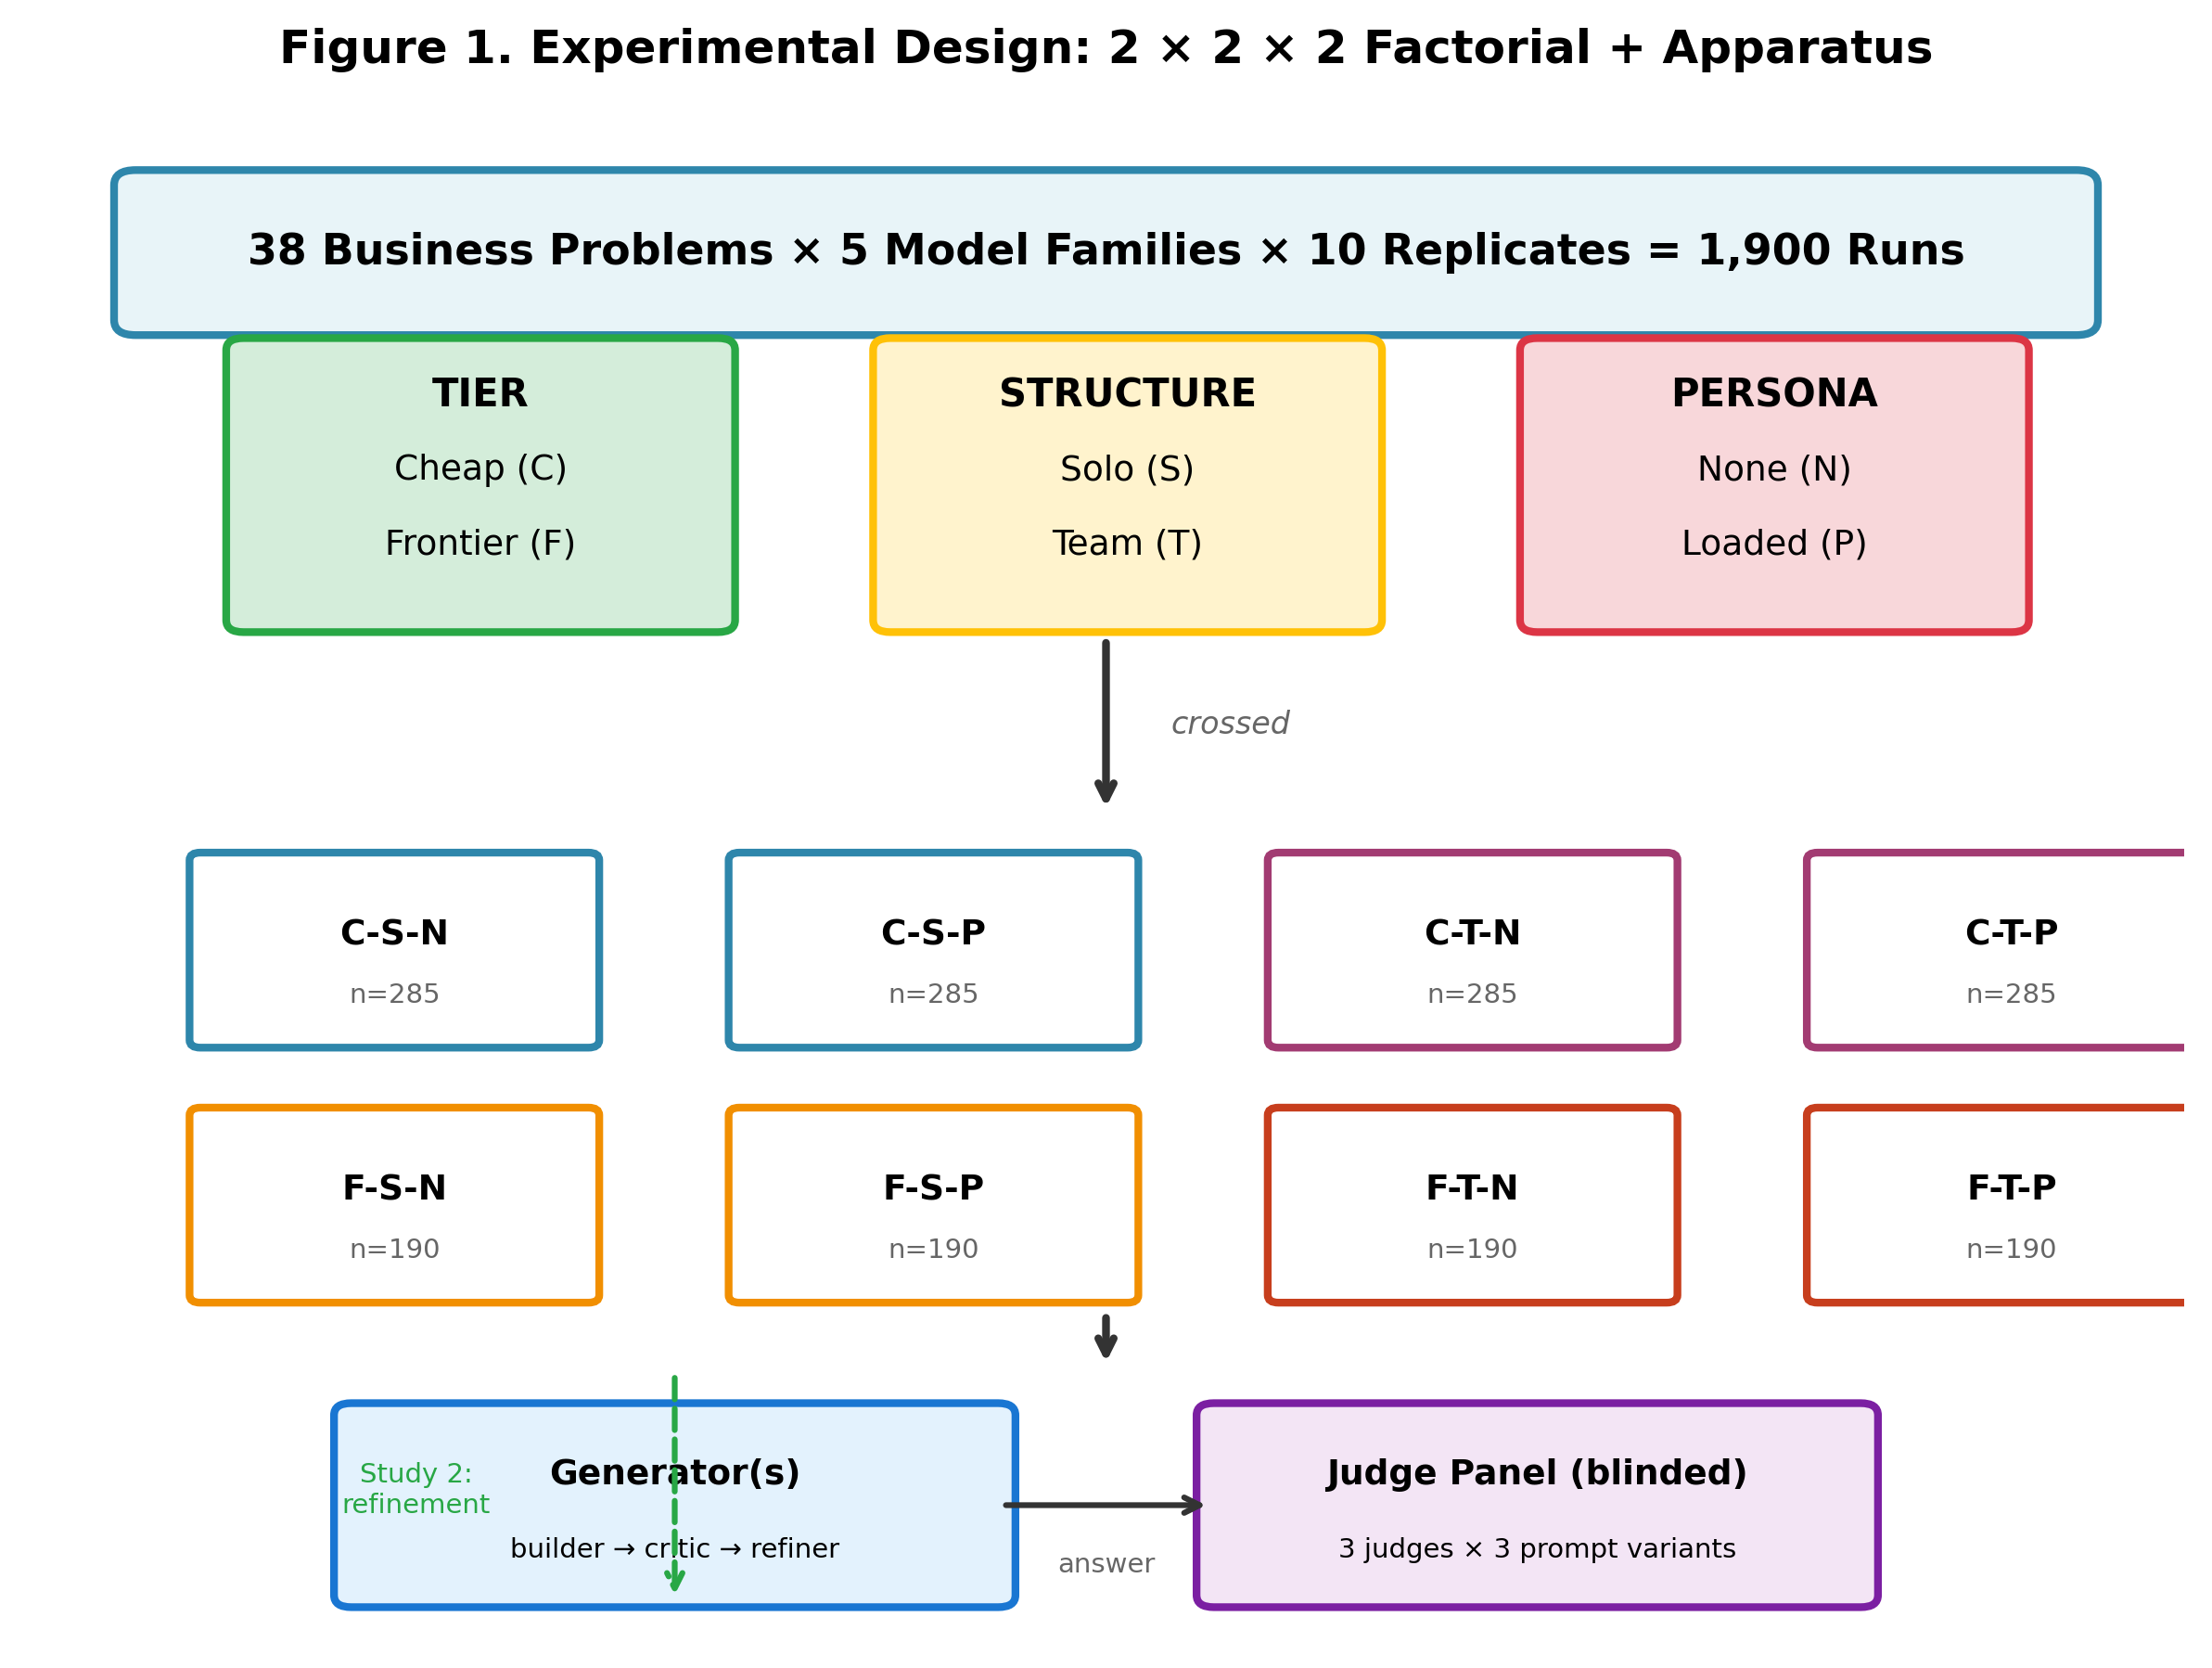
\includegraphics[width=\textwidth]{figures/fig1_design_schematic.png}
  \caption{Experimental Design: $2 \times 2 \times 2$ Factorial + Apparatus.}
  \label{fig:design}
\end{figure}

\subsection{Models Evaluated}\label{sec:models}

\subsubsection{Frontier Models (Five Families)}

Each family contributes its current \emph{mainline} flagship, pinned on
2026-07-30: \texttt{kimi-k3}, \texttt{qwen3.7-max-2026-06-08},
\texttt{gpt-5.6-sol}, \texttt{claude-opus-5}, and
\texttt{gemini-3.1-pro-preview}. Above-mainline tiers (e.g.\
\texttt{claude-fable-5}) are deliberately excluded because they would break
cross-family comparability. Gemini's preview status carries a pre-registered
fallback to \texttt{gemini-2.5-pro} if the model is retired mid-experiment; the
fallback was never invoked. All models run with generator temperature $= 1$, a
uniform value forced by the OpenAI and Moonshot APIs (which reject other values)
and applied identically across families for \emph{ceteris paribus}
comparability~(D27).

\subsubsection{Cheap Siblings}

Each family contributes one cheap-tier model from the same generation:
\texttt{kimi-k2.6}, \texttt{qwen3.7-plus-2026-05-26}, \texttt{gpt-5.6-luna},
\texttt{claude-haiku-4-5-20251001}, and \texttt{gemini-3.1-flash-lite}. Price
ratios (frontier : cheap) range from 3.4$\times$ to 8$\times$ across families.
Family-level heterogeneity in price ratio is absorbed by the family random
effect in our mixed-model analysis (\cref{sec:inferential}); it is not a
confound of the primary tier $\times$ structure test.

\subsection{Orchestration Structures and Personas}

\textbf{Solo} runs invoke a single model call on the rendered problem.
\textbf{Team} runs execute a three-step pipeline --- builder produces a draft,
critic critiques it, refiner produces the final answer --- with all intermediate
outputs discarded from the judged answer (and therefore from the quality score)
but retained in the cost ledger (a disclosed cost bias, favorable to the
cheap-team cells). Persona is implemented as a fixed mapping from role
(builder/critic/refiner) to a cultural persona description, identical across all
problems and families \citep{Hariri2026b}. The mapping is pre-registered and
never varied per-problem; it is therefore a treatment level, not a confound.

\subsection{Stimuli and Response Generation}

Thirty-eight domain-stratified business problems are used. Fifteen are inherited
verbatim from a prior validated set \citep{Hariri2025a}; ten were drafted
post-cutoff to control for contamination and validated as structurally identical;
the remainder extend the grid to cover five domains equally. Each problem is
rendered as \texttt{background\_context + "\textbackslash n\textbackslash n" +
business\_problem} with no instructional wrapper --- adding wrapper text would
introduce an unmeasured prompt treatment. Generator temperature is fixed at~1
(\cref{sec:models}). Every run is time-stamped and flagged for whether it
executed inside the pre-registered preferred window (14:00--00:00 UTC), which
simultaneously captures the Qwen off-peak discount and fully avoids both
DeepSeek peak-surge windows; window-free providers (Kimi, Together-hosted
models, Western providers) are time-invariant and therefore unaffected.

\subsection{Evaluation Framework}\label{sec:eval}

\subsubsection{Judge Model Selection}

Three judges from families disjoint from every generator: \texttt{deepseek-chat}
(resolved to \texttt{deepseek-v4-flash}), \texttt{zai-org/GLM-5.2}, and
\texttt{meta-llama/Llama-3.3-70B-Instruct-Turbo}. The disjointness rule~(D33)
guards against self-enhancement bias \citep{ZhengEtAl2023}: even when deepseek
is the registered fallback generator, the fallback was never invoked, so
disjointness holds in the executed data.

\subsubsection{Scoring Rubric}

Six 1--5 dimensions are scored: \textbf{Novelty, Usefulness, Flexibility,
Elaboration, Cultural Sensitivity, and an aggregate Practicality}. The composite
primary outcome is the mean of the first five dimensions. Three prompt variants
are used per judge, frozen verbatim and never re-optimized after a prior
judge-prompt optimization attempt collapsed $\kappa$ in earlier work
\citep{Hariri2025a}. Every solution is scored by all three judges under all
three variants (nine scores per solution), with candidate order shuffled per
variant to neutralize position bias \citep{ZhengEtAl2023}. Judges run at
temperature~0 for determinism.

\subsubsection{Inter-Rater Reliability}

Pairwise judge correlations on per-run composite scores are 0.87
(deepseek--zhipu), 0.61 (deepseek--meta), and 0.49 (meta--zhipu). The
panel-level reliability exceeds any single judge's correlation with the latent
quality; this mirrors the jury logic of \citet{VergaEtAl2024} in which diversity
of smaller judges outperforms a single large judge.

\subsection{Statistical Analysis}

\subsubsection{Effect Sizes}

Welch's $d$ with bootstrap 95\% confidence intervals (5{,}000 resamples, seed
42) throughout \citep{Lakens2013}. Estimation-first reporting: intervals, not
$p$-values, carry the weight of the argument; $p$-values are reported for
completeness and to comply with sequential-analysis boundaries
(\cref{sec:inferential}).

\subsubsection{Inferential Statistics}\label{sec:inferential}

The primary test of $H_1$ is the pre-registered interaction contrast
$d = (FT - FS) - (CT - CS)$, expected negative (team helps cheap more than
frontier). Inference uses a mixed model with random effects for \emph{problem}
and \emph{family}, solving the pseudo-replication identified in the author's
prior work \citep{Hariri2026b}. Sequential analysis with an O'Brien--Fleming
spending function (protocol~03) governs interim looks and the final stopping
boundary; the Bayesian JZS Bayes factor is reported as recommended (A2.4) but
does not gate the decision. Family-wise corrections within secondary hypotheses
use Benjamini--Hochberg FDR ($\alpha = 0.05$); Holm is used for the small set of
directional family comparisons in Study~2.

\subsubsection{Economic Analysis}

Cost is stored as tokens in a run-level ledger and re-priced through a frozen
price vector (\texttt{config/price\_vector.json}, version 2026-07-30). Because
the ledger does not split input from output tokens, cost is computed under a
blended price $\mathrm{blend}(\phiBlend) = \phiBlend \cdot p_{\mathrm{out}} +
(1 - \phiBlend) \cdot p_{\mathrm{in}}$ with a primary $\phiBlend = 0.50$ and a
sensitivity panel $\phiBlend \in \{0.25, 0.50, 0.75\}$ (\citealt{Diewert1976}
provides the price--quantity decomposition precedent; \citealt{SteegenEtAl2016}
the multiverse-robustness precedent). Frontier-membership claims must be stable
across all three $\phiBlend$. The \textbf{Tiered Efficiency Gain Ratio (T-EGR)}
is $(\mathrm{Quality}_{\mathrm{cell}} / \mathrm{Quality}_{F\text{-}S\text{-}N})
/ (\mathrm{Cost}_{\mathrm{cell}} / \mathrm{Cost}_{F\text{-}S\text{-}N})$,
computed within each family and pooled; F-S-N is the baseline. \textbf{ICER} is
reported relative to the cheapest cell. Judge cost is excluded from unit T-EGR
(it is shared infrastructure, not cell compute; a disclosed exclusion).

\subsubsection{Robustness Checks}

Pre-registered battery~(A2): leave-one-family-out, leave-one-problem-out,
mean-vs-median, BH-FDR on secondary dimensions, length-confound adjustment on
$H_1$, and empirical-Bayes partial pooling of per-family interaction estimates.
Random-effects meta-analysis across the five families confirms the interaction
generalizes (pooled $d = -0.270$, $I^2 = 28.5\%$).

\subsubsection{Qualitative Coding Protocol (Study~2)}\label{sec:qual-coding}

Thirty triples (original CTP / refined CTP / same-problem same-family FSN) are
sampled deterministically (seed 20260801, 10 per family). Two blinded LLM coders
perform a two-wave coding: free induction on a subset, then closed coding
against a frozen 13-code codebook (six RQ1 insight codes, six RQ2 structure
codes, one RQ3 bloat code). Cohen's $\kappa$ gate is 0.70; codes below threshold
are downgraded to medium reliability and disclosed \citep{Cohen1960}. The prompt
presented to coders contains the three texts only --- no cell label, family, or
score, preserving blind evaluation.

\subsection{Validity and Reliability}

\textbf{Construct validity:} the rubric separates Novelty from
Usefulness/Elaboration, so a stylistic shift (e.g.\ more discourse markers from
a persona) is not conflated with substantive quality. \textbf{Internal validity:}
frozen configurations, blinded judging, shuffled order, disjoint judge families.
\textbf{External validity:} single task domain (English business strategy) is
the acknowledged boundary. \textbf{Disclosed threats:} intermediate team outputs
excluded from judged answers bias team costs downward (favorable to cheap teams,
disclosed not corrected); truncation at source affects a small set of long runs
and is audited separately.

\subsection{Code and Data Availability}

All analysis code, the frozen token ledger, judge rationales, and the ten
protocols are committed to the \texttt{orchestration-economics} repository; the
OSF registration is \texttt{osf.io/mjb8x}. A reproduction runbook
\citep{SandveEtAl2013} lists the commands that regenerate every number reported
in~\cref{sec:results}.

\subsection{AI-Assisted Research Disclosure}\label{sec:ai-disclosure}

This study used large language models as research tools under continuous human
supervision. Specifically, \textbf{Kimi} (Moonshot AI, \texttt{kimi-k3}) and
\textbf{Qwen} (Alibaba Cloud, \texttt{qwen3.7-max}) were employed in the
following capacities: (1)~\textbf{ideation} --- brainstorming experimental
design alternatives, hypothesis formulations, and analysis strategies during the
protocol-drafting phase; (2)~\textbf{code generation} --- producing initial
versions of the execution pipeline, statistical analysis scripts, and
figure-generation code, all of which were reviewed, corrected, and approved by
the author before execution; (3)~\textbf{audit} --- reviewing citation accuracy,
checking statistical assumptions, and identifying inconsistencies across
protocol documents; (4)~\textbf{execution} --- running the generation and
judging campaigns through API calls, with all configurations frozen and logged
before each run.

No LLM made unsupervised decisions about the experimental design, statistical
analysis, or the interpretation of results. All ten pre-registered protocols,
all 39 design decisions (D1--D39), and all analysis choices were authored,
reviewed, and approved by the human author. LLM-generated code was treated as a
first draft, not a final product: every script was inspected, every output was
validated against expected ranges, and every reported number traces to a frozen,
version-controlled analysis pipeline. The qualitative coding protocol
(\cref{sec:qual-coding}) used two LLM coders with blinded evaluation --- a
design choice that converts the LLM's systematic biases into a measured
inter-rater reliability coefficient ($\kappa = 0.824$) rather than an unmeasured
confound.

The use of LLMs as evaluation judges (\cref{sec:eval}) is a distinct
methodological choice from the use of LLMs as research tools: the judges
evaluate \emph{generated business solutions}, not the research process itself.
The disjointness rule~(D33) ensures that no judge shares architecture with any
generator, mitigating the self-enhancement bias documented by
\citet{ZhengEtAl2023}.

% ==================================================================
% 4  RESULTS
% ==================================================================
\section{Results}\label{sec:results}

\subsection{The Interaction Effect: Does Pipeline Structure Pay Off More for
Cheap Models?}\label{sec:interaction}

From a resource-allocation perspective, the most important finding is that
pipeline structure delivers higher marginal returns at the cheap tier than at
the frontier tier. The pre-registered interaction contrast is $d = -0.227$
(bootstrap 95\% CI $[-0.410, -0.040]$, Welch $t = -2.45$, $p = 0.0145$), with
the sequential-analysis boundary crossed at the scheduled final look. For a
firm making an AI budget decision, this implies that pipeline dollars are better
spent upgrading cheap models to team configurations than adding team overhead to
already-expensive frontier models. The JZS Bayes factor for the interaction is
1.002 (inconclusive), reported as recommended but not gating the decision.

The secondary effects provide additional strategic context. The \textbf{tier
main effect} ($d = +0.294$, CI $[+0.201, +0.382]$, $\BF_{10} = 1.7 \times
10^7$) confirms that frontier models command a quality premium, but the
magnitude is dwarfed by the cost difference. The \textbf{structure main effect}
($d = +0.117$, CI $[+0.030, +0.205]$) shows that teams slightly outperform
solos on average --- a small but consistent productivity gain from
orchestration. The \textbf{persona main effect} is large and in the
\emph{opposite} direction to the pre-registered expectation: $d = -0.691$ (CI
$[-0.761, -0.620]$, $\BF_{10} = 1.0 \times 10^{50}$). Persona-loaded cells
score \emph{lower} than their no-persona twins, representing a failed
investment in stylistic differentiation. From a business perspective, personas
increase cost while degrading output quality --- a value-destroying
configuration. A post-hoc dimension decomposition shows that Novelty is the sole
dimension where personas help (+0.154, $p_{\mathrm{FDR}} = 0.001$) while
Usefulness ($-1.024$) and Elaboration ($-0.966$) drive the reversal. The
structure $\times$ persona interaction is not significant ($F = 1.23$, $p =
0.27$).

\begin{quote}
\textbf{Strategic Implication:} Pipeline structure is a cheap-tier amplifier,
not a universal substitute. For budget-constrained firms, investing in team
pipelines for cheap models yields the highest marginal return. Personas, by
contrast, represent value destruction --- they increase cost while degrading
quality.
\end{quote}

\begin{figure}[ht]
  \centering
  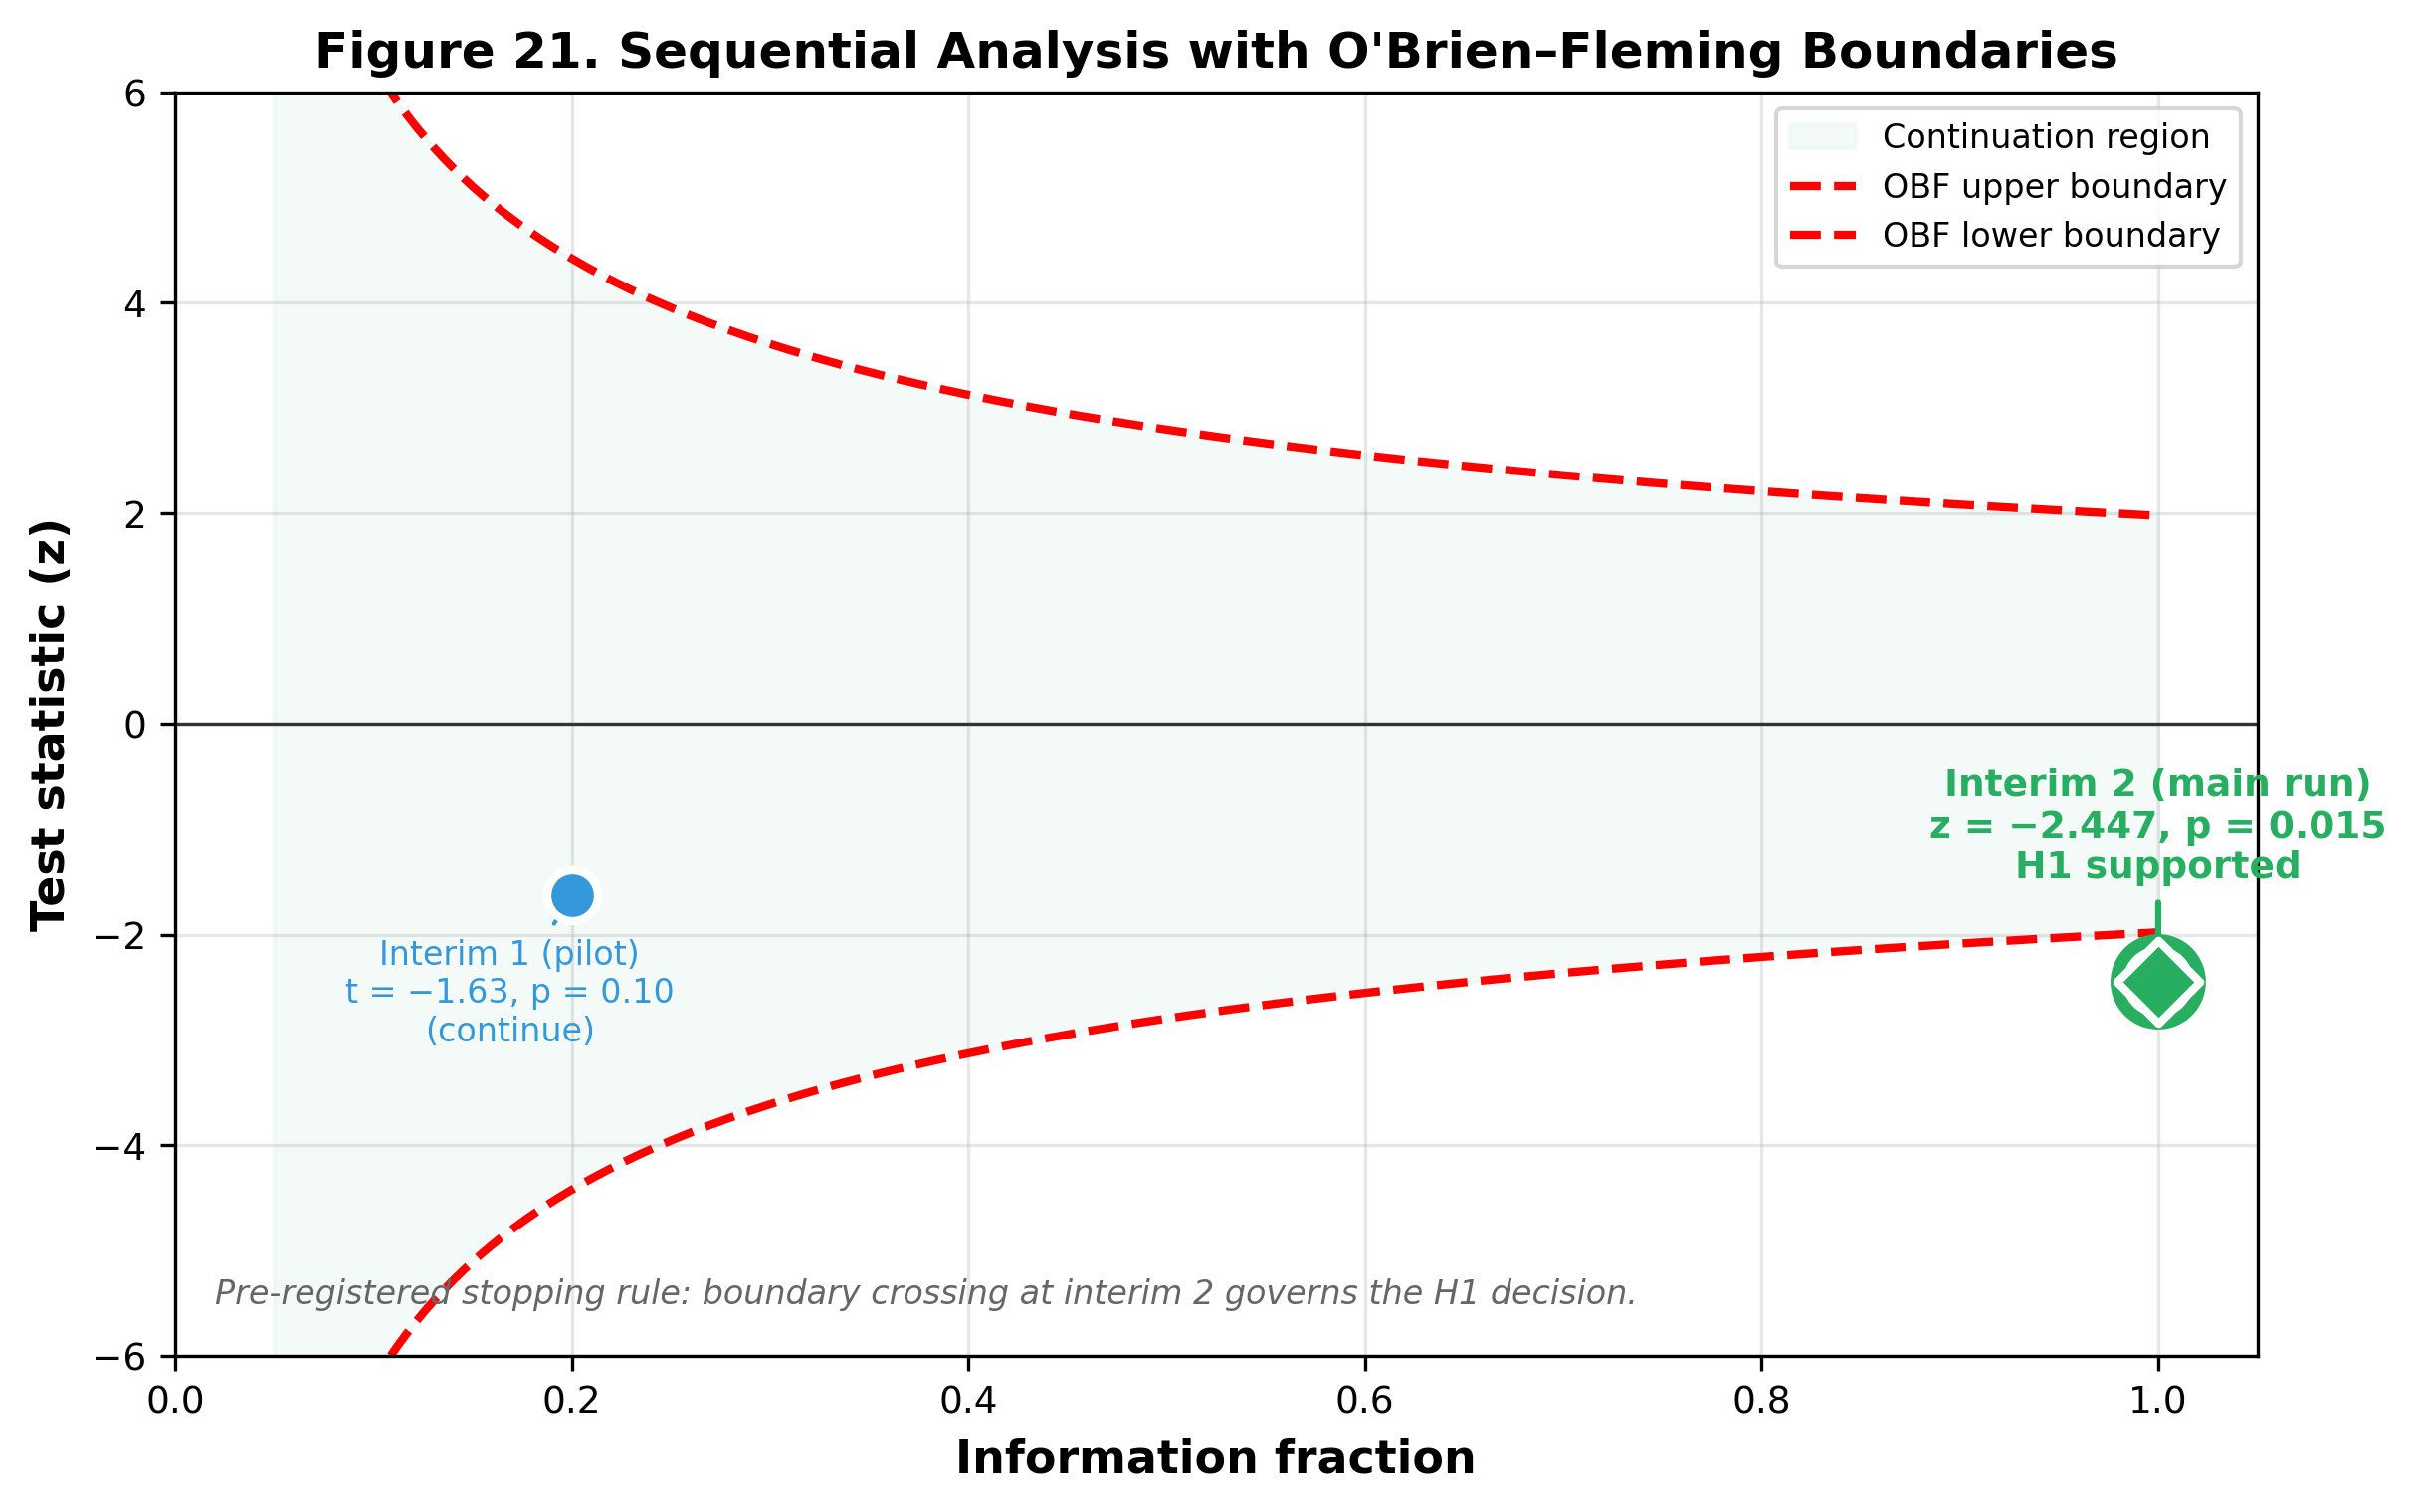
\includegraphics[width=\textwidth]{figures/fig21_sequential_boundary.png}
  \caption{Sequential analysis with O'Brien--Fleming spending function. The test
    statistic $z = -2.447$ crosses the interim-2 boundary $|z| \ge 1.977$
    (dashed line). The shaded region is the continuation region. The
    pre-registered decision is to stop and report $H_1$ as supported.}
  \label{fig:sequential}
\end{figure}

\begin{figure}[ht]
  \centering
  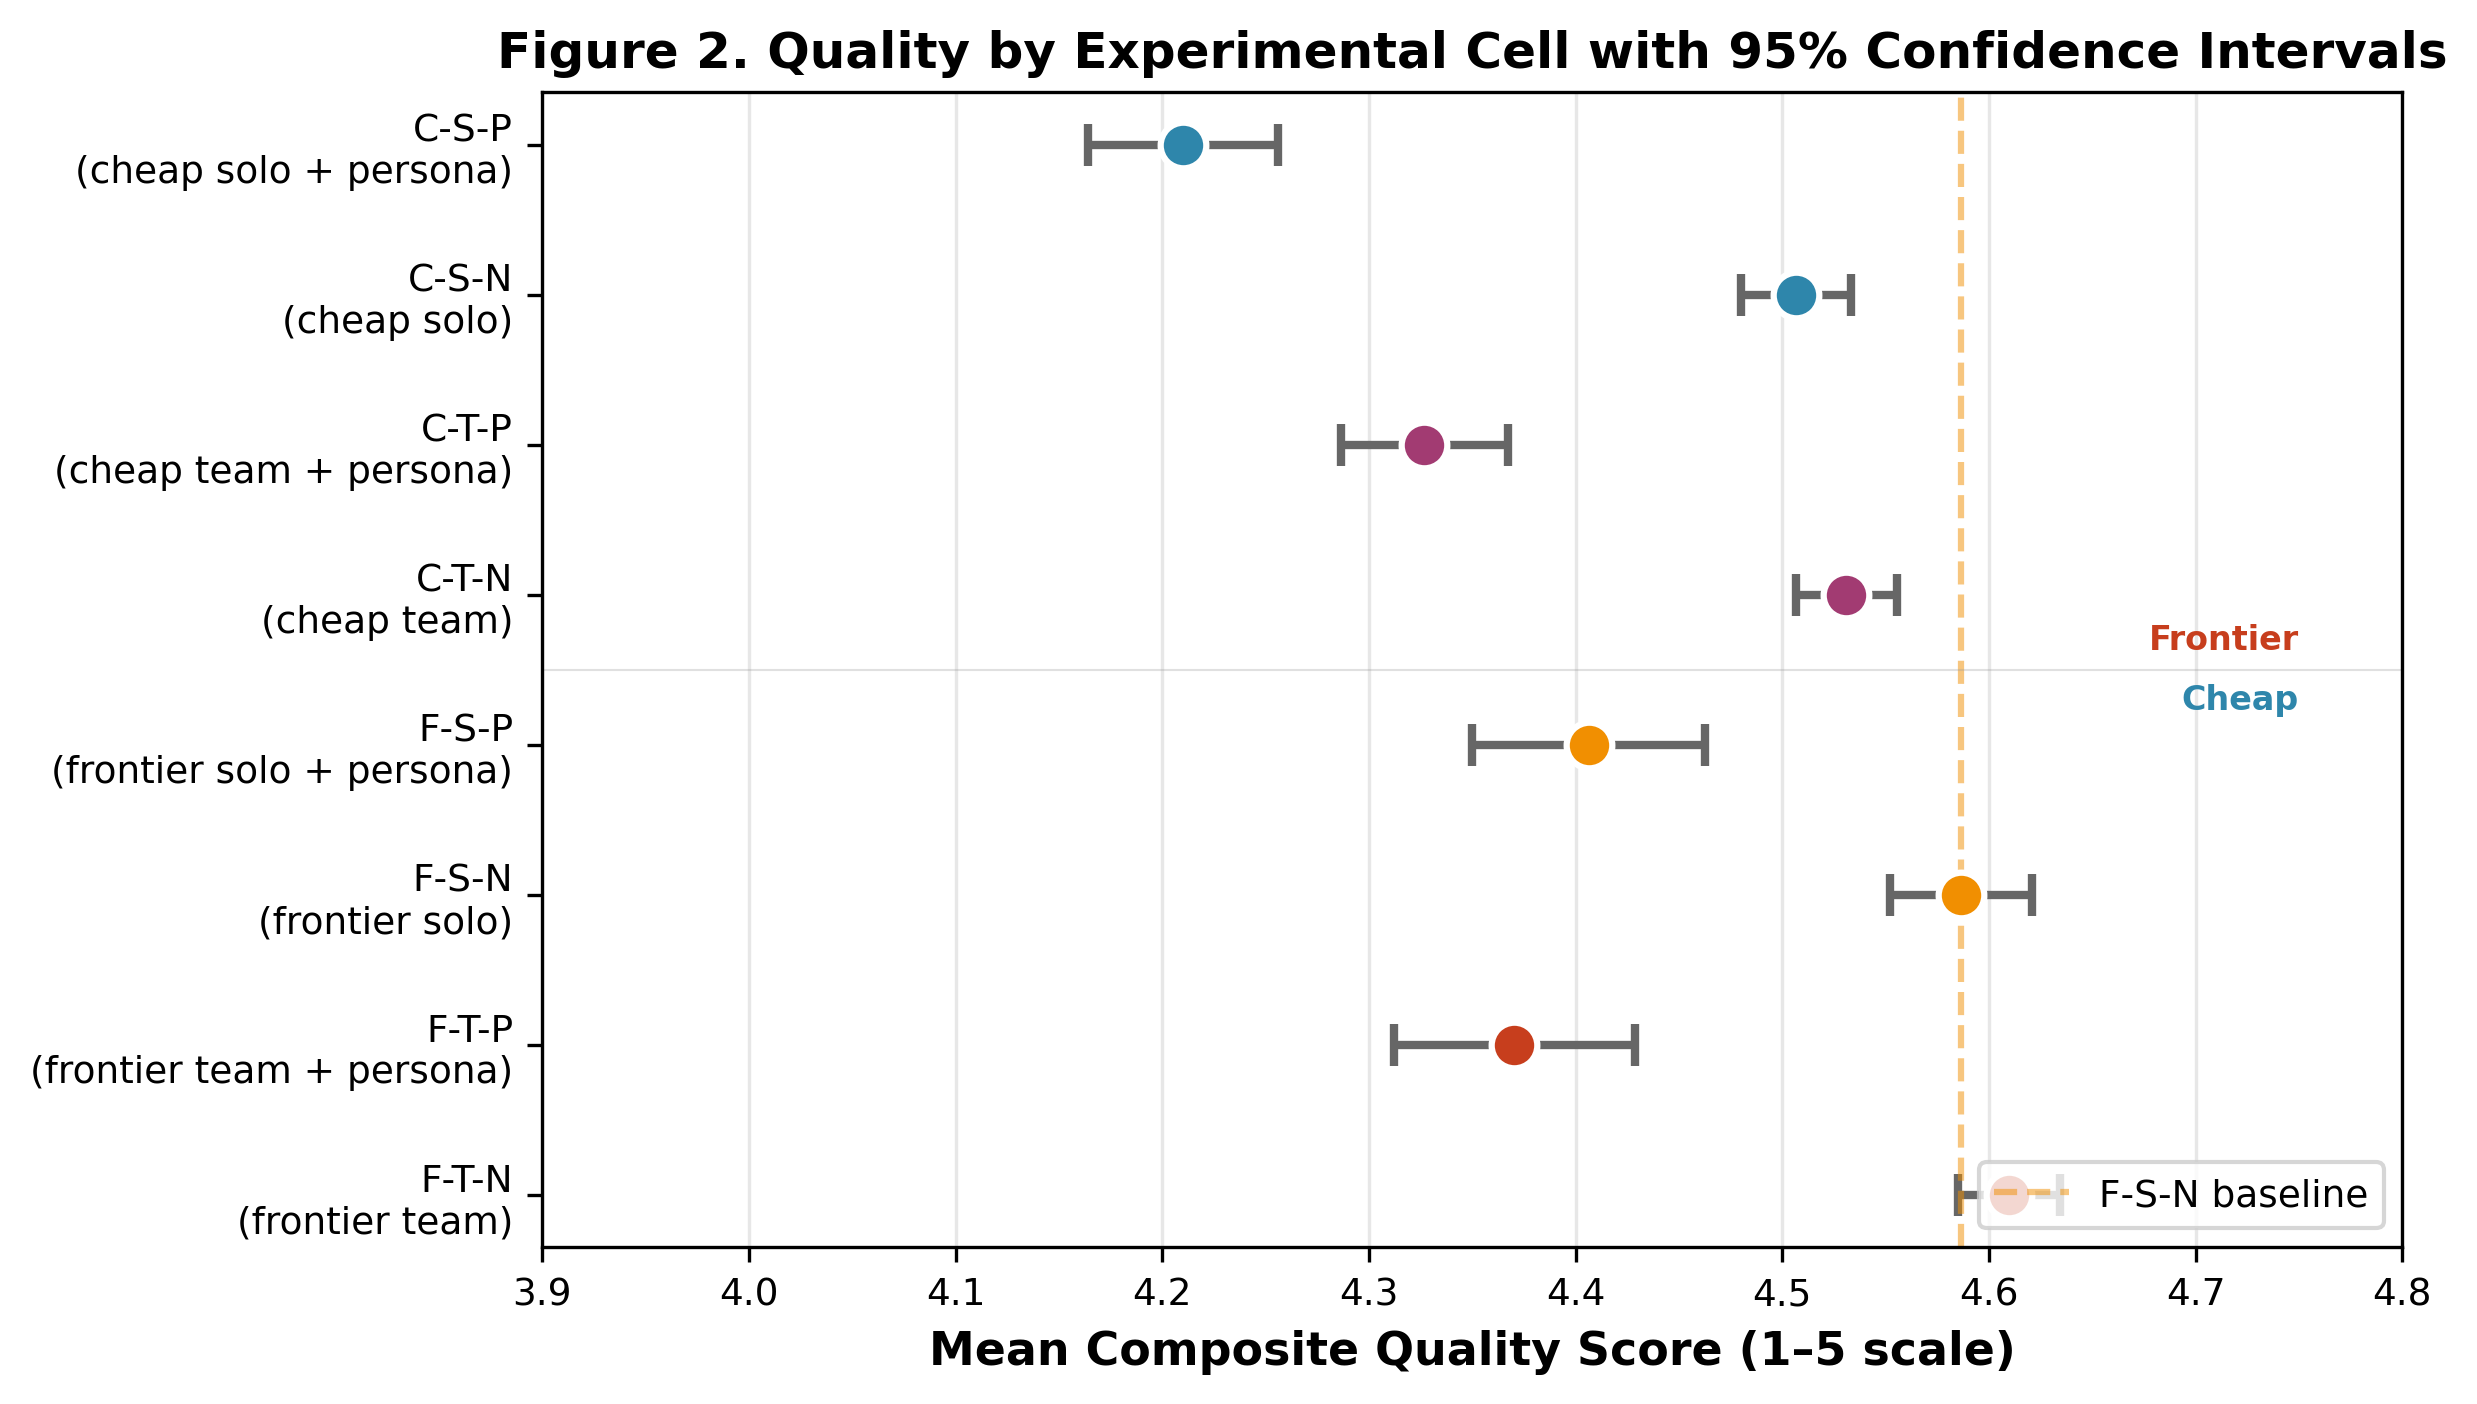
\includegraphics[width=\textwidth]{figures/fig2_forest_plot.png}
  \caption{Quality by Experimental Cell with 95\% Confidence Intervals.}
  \label{fig:forest}
\end{figure}

\subsection{The Hidden Cost of Personas: Style Without Substance}\label{sec:persona-penalty}

Every persona-loaded cell is Pareto-dominated by its no-persona twin on the
cost--quality plane: at equal or lower cost, the N~cell scores higher on
composite quality. The penalty is largest on dimensions that rubric readers
associate with substance (Usefulness, Elaboration), smallest on the one most
susceptible to stylistic signaling (Novelty). This pattern mirrors the
contingency finding in the author's prior work \citep{Hariri2026b} and is
consistent with the jagged-frontier mechanism \citep{DellAcquaEtAl2023}:
personas push the generator toward a more stylized region of its output space
that the judge, correctly, penalizes on substance.

\begin{quote}
\textbf{Strategic Implication:} Personas degrade output quality while increasing
cost --- they are value-destroying for knowledge-work tasks. Firms should treat
them as a failed investment rather than a quality lever.
\end{quote}

\begin{figure}[ht]
  \centering
  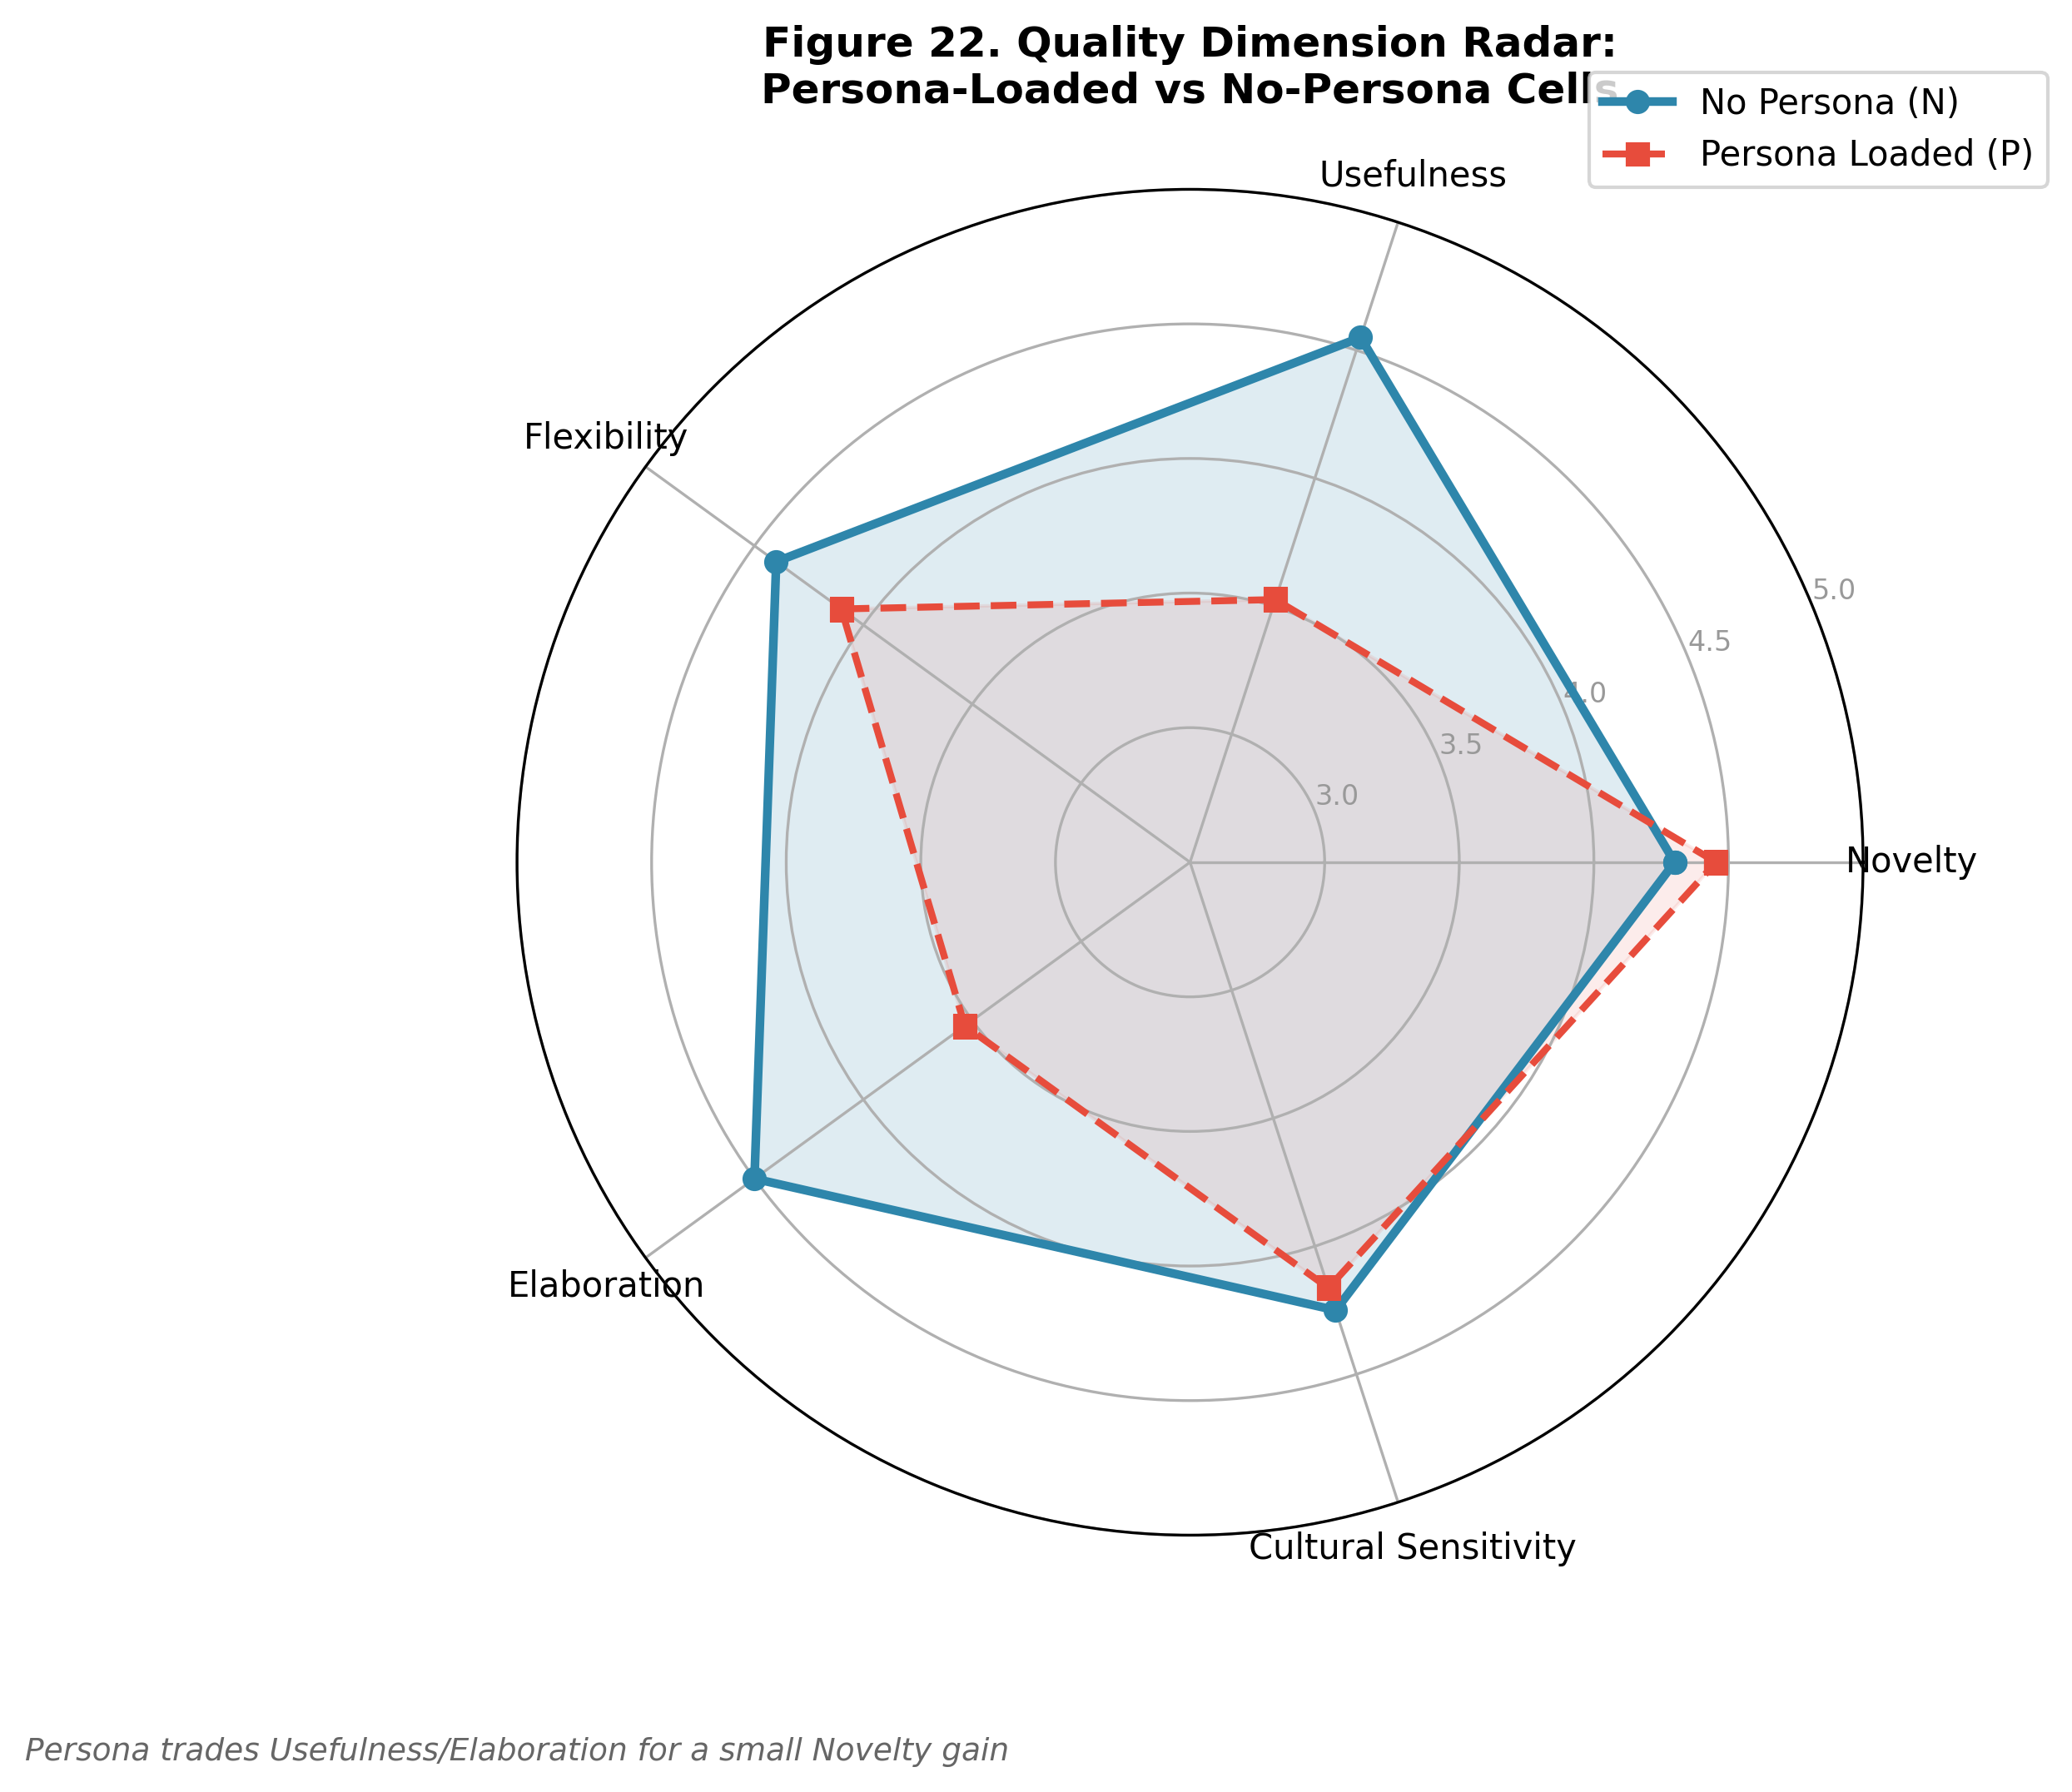
\includegraphics[width=0.85\textwidth]{figures/fig22_persona_radar.png}
  \caption{Quality-dimension radar for persona-loaded (red, dashed) versus
    no-persona (blue, solid) cells. The persona polygon is visibly smaller on
    Usefulness and Elaboration, slightly larger on Novelty --- the visual
    signature of the style-over-substance tradeoff.}
  \label{fig:persona-radar}
\end{figure}

\begin{figure}[ht]
  \centering
  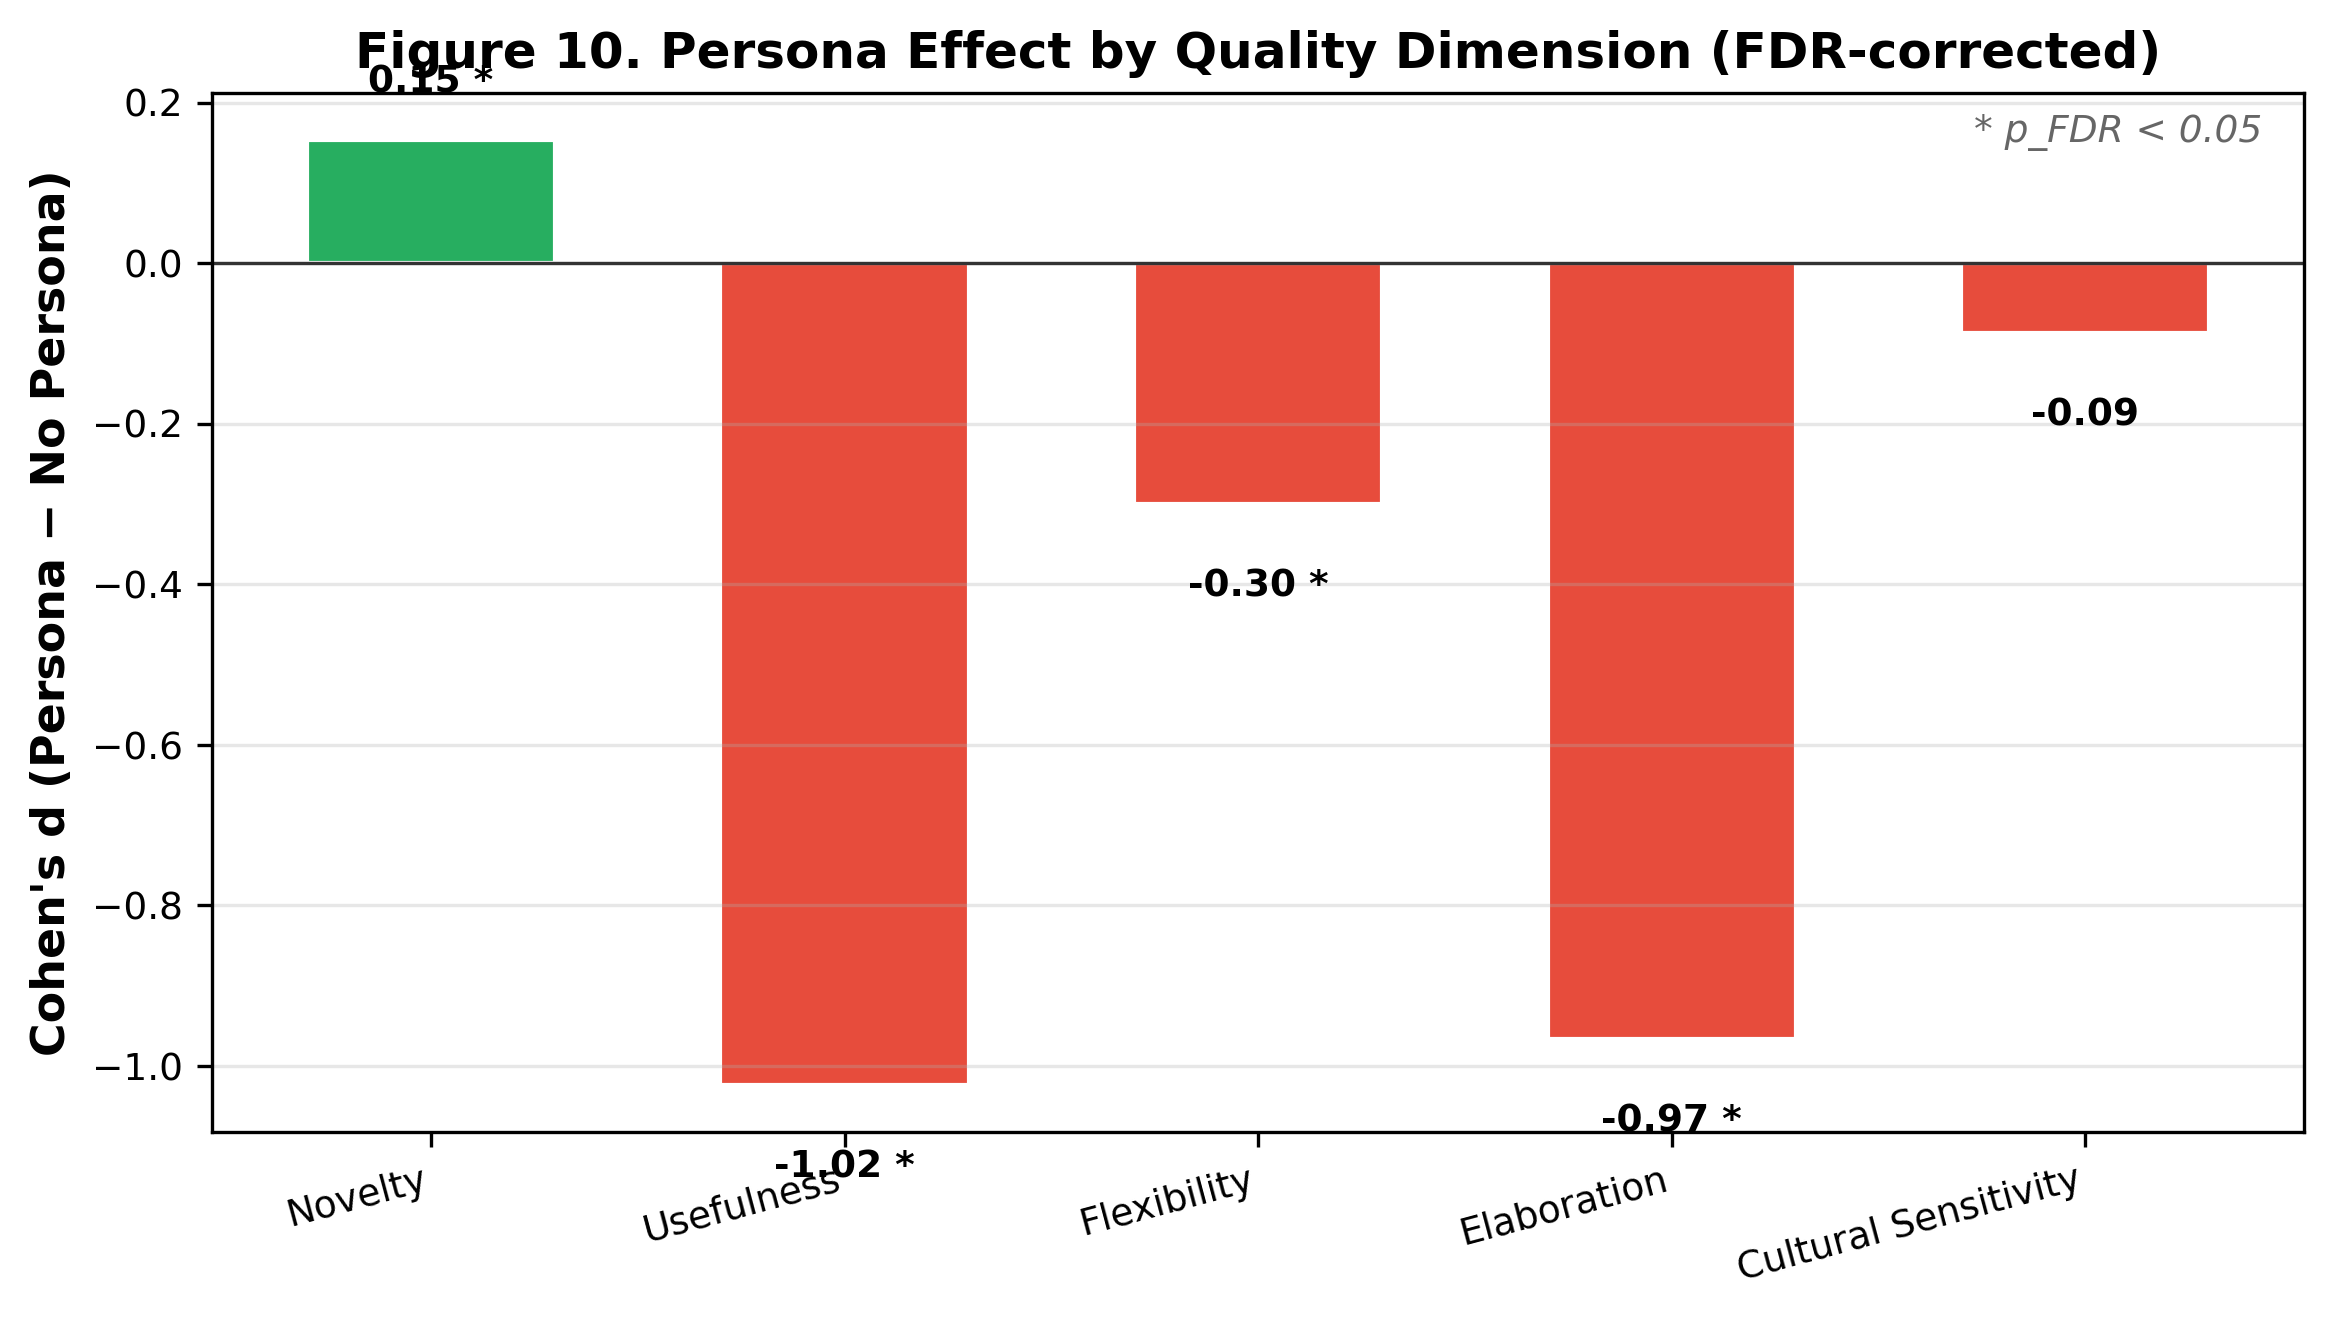
\includegraphics[width=\textwidth]{figures/fig10_persona_dimensions.png}
  \caption{Persona Effect by Quality Dimension (FDR-Corrected).}
  \label{fig:persona-dims}
\end{figure}

\subsection{The Frontier Gap: Can Cheap Teams Match Frontier Performance?}\label{sec:frontier-gap}

Paired comparisons between cheap-team-with-persona (CTP) and the
frontier-solo-no-persona baseline (F-S-N) are negative in all five families
(kimi $d = -0.71$, claude $d = -1.42$, qwen $d = -2.17$; all CIs exclude zero
after Holm correction). The gap is the empirical target that a refinement pass
must close --- the question of Study~2.

\begin{quote}
\textbf{Strategic Implication:} As executed, cheap teams do not beat a single
frontier call on matched problems. The substitution thesis is bounded: structure
improves cheap models but cannot fully close the frontier gap without additional
investment.
\end{quote}

\subsection{The Refinement Play: Closing the Gap at Low Marginal Cost}\label{sec:refinement}

A frozen, add-only refiner is applied to the CTP outputs. The pilot satisfied
the feasibility gate (G1, 100\% completion); the full-pool extension covered 171
pairs per family. The pre-registered superiority gate (G2: $d \ge 0.2$ with CI
excluding~0 in all three families, in the direction refined $>$ FSN) is
mechanically failed in all three families: kimi $d = -0.295$, claude $d =
-1.301$, qwen $d = -0.809$ (all CIs strictly negative after Holm). The
superiority claim is formally rejected.

Refinement nevertheless does substantial repair work. Measured as gap recovery
against each family's own pre-refinement CTP-vs-FSN gap, the pass recovers 60\%
of the gap for kimi, 8\% for claude (whose pre-refinement gap was already
small), and 64\% for qwen. The Novelty protection criterion (H2.2: no family
loses more than $-0.10$ Novelty) is passed by all three; Novelty actually
\emph{increases} for qwen ($d = 1.10$, $p_{\mathrm{FDR}} < 0.001$). Usefulness
and Elaboration show large gains in kimi and qwen ($d = 0.8$ to $1.4$, all
$p_{\mathrm{FDR}} < 0.001$) and are unchanged in claude --- which was already at
ceiling on those dimensions before refinement.

Length analysis confirms the dilution hypothesis is \emph{not} the driver: the
pooled Pearson correlation between length ratio (refined/original) and
composite-score change is $r = +0.68$, Spearman $\rho = +0.71$ ($p < 0.001$).
Longer refined answers score higher, not lower.

Cross-family comparisons (\cref{fig:cross-family}) remain negative after
refinement: no cross-family CTP pairing flips to superiority, confirming that
the within-family result is not an artifact of family selection.

\begin{quote}
\textbf{Strategic Implication:} A \$0.002 refinement pass delivers bounded
improvement --- it recovers most of the frontier gap on average but never
achieves paired superiority. For firms, this means refinement is a viable
risk-mitigation strategy (improve quality cheaply) but not a replacement
strategy (it will not beat the frontier).
\end{quote}

\begin{figure}[ht]
  \centering
  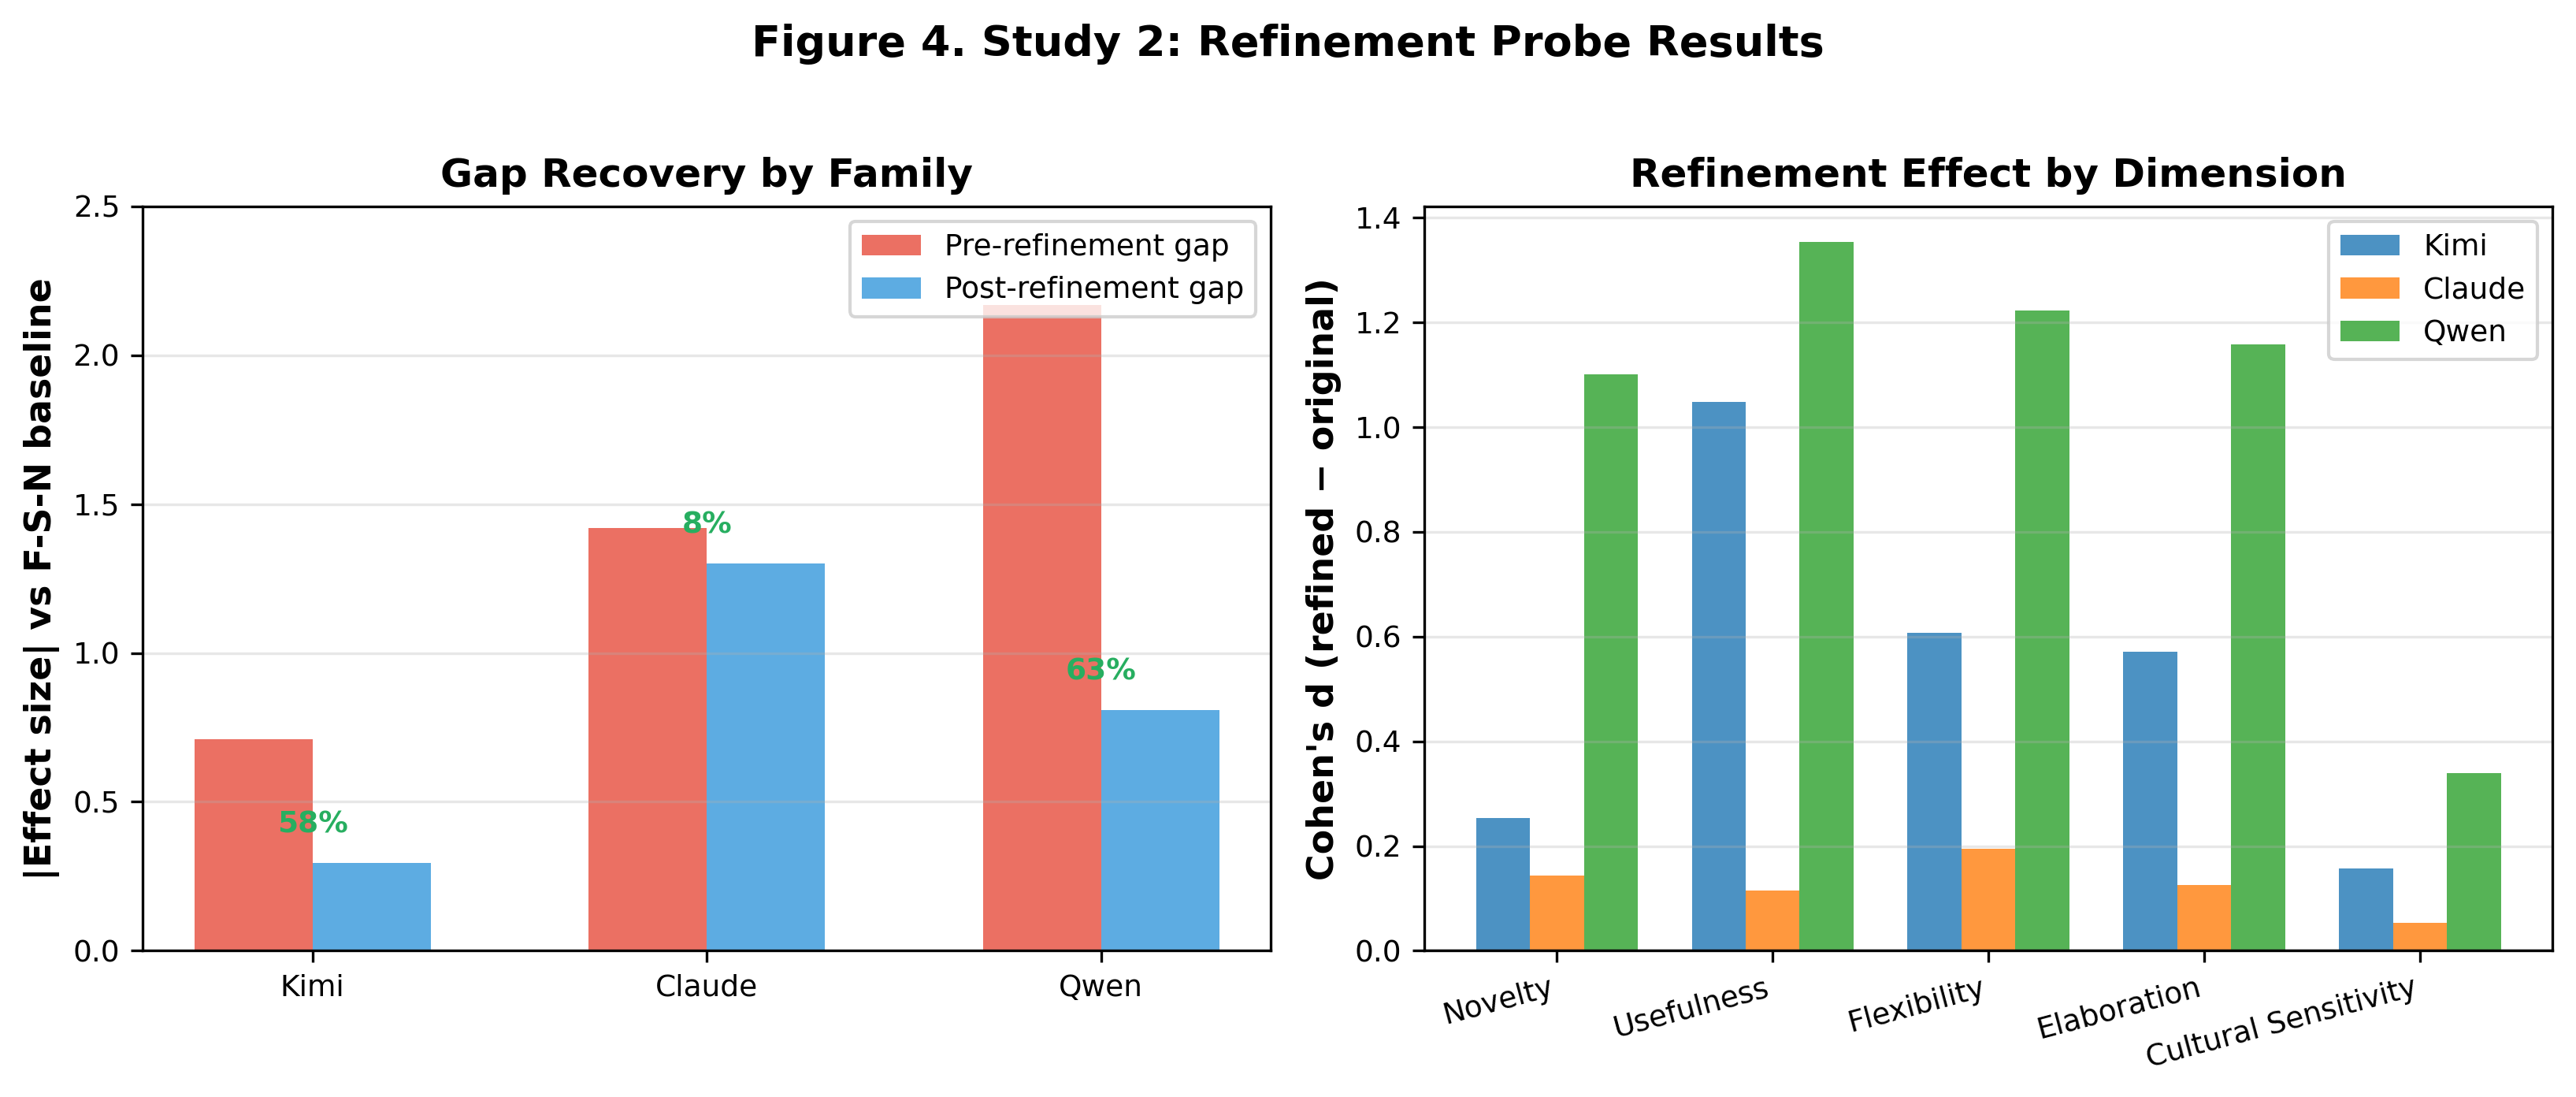
\includegraphics[width=\textwidth]{figures/fig4_gap_recovery.png}
  \caption{Study~2: Refinement Probe Results.}
  \label{fig:gap-recovery}
\end{figure}

\begin{figure}[ht]
  \centering
  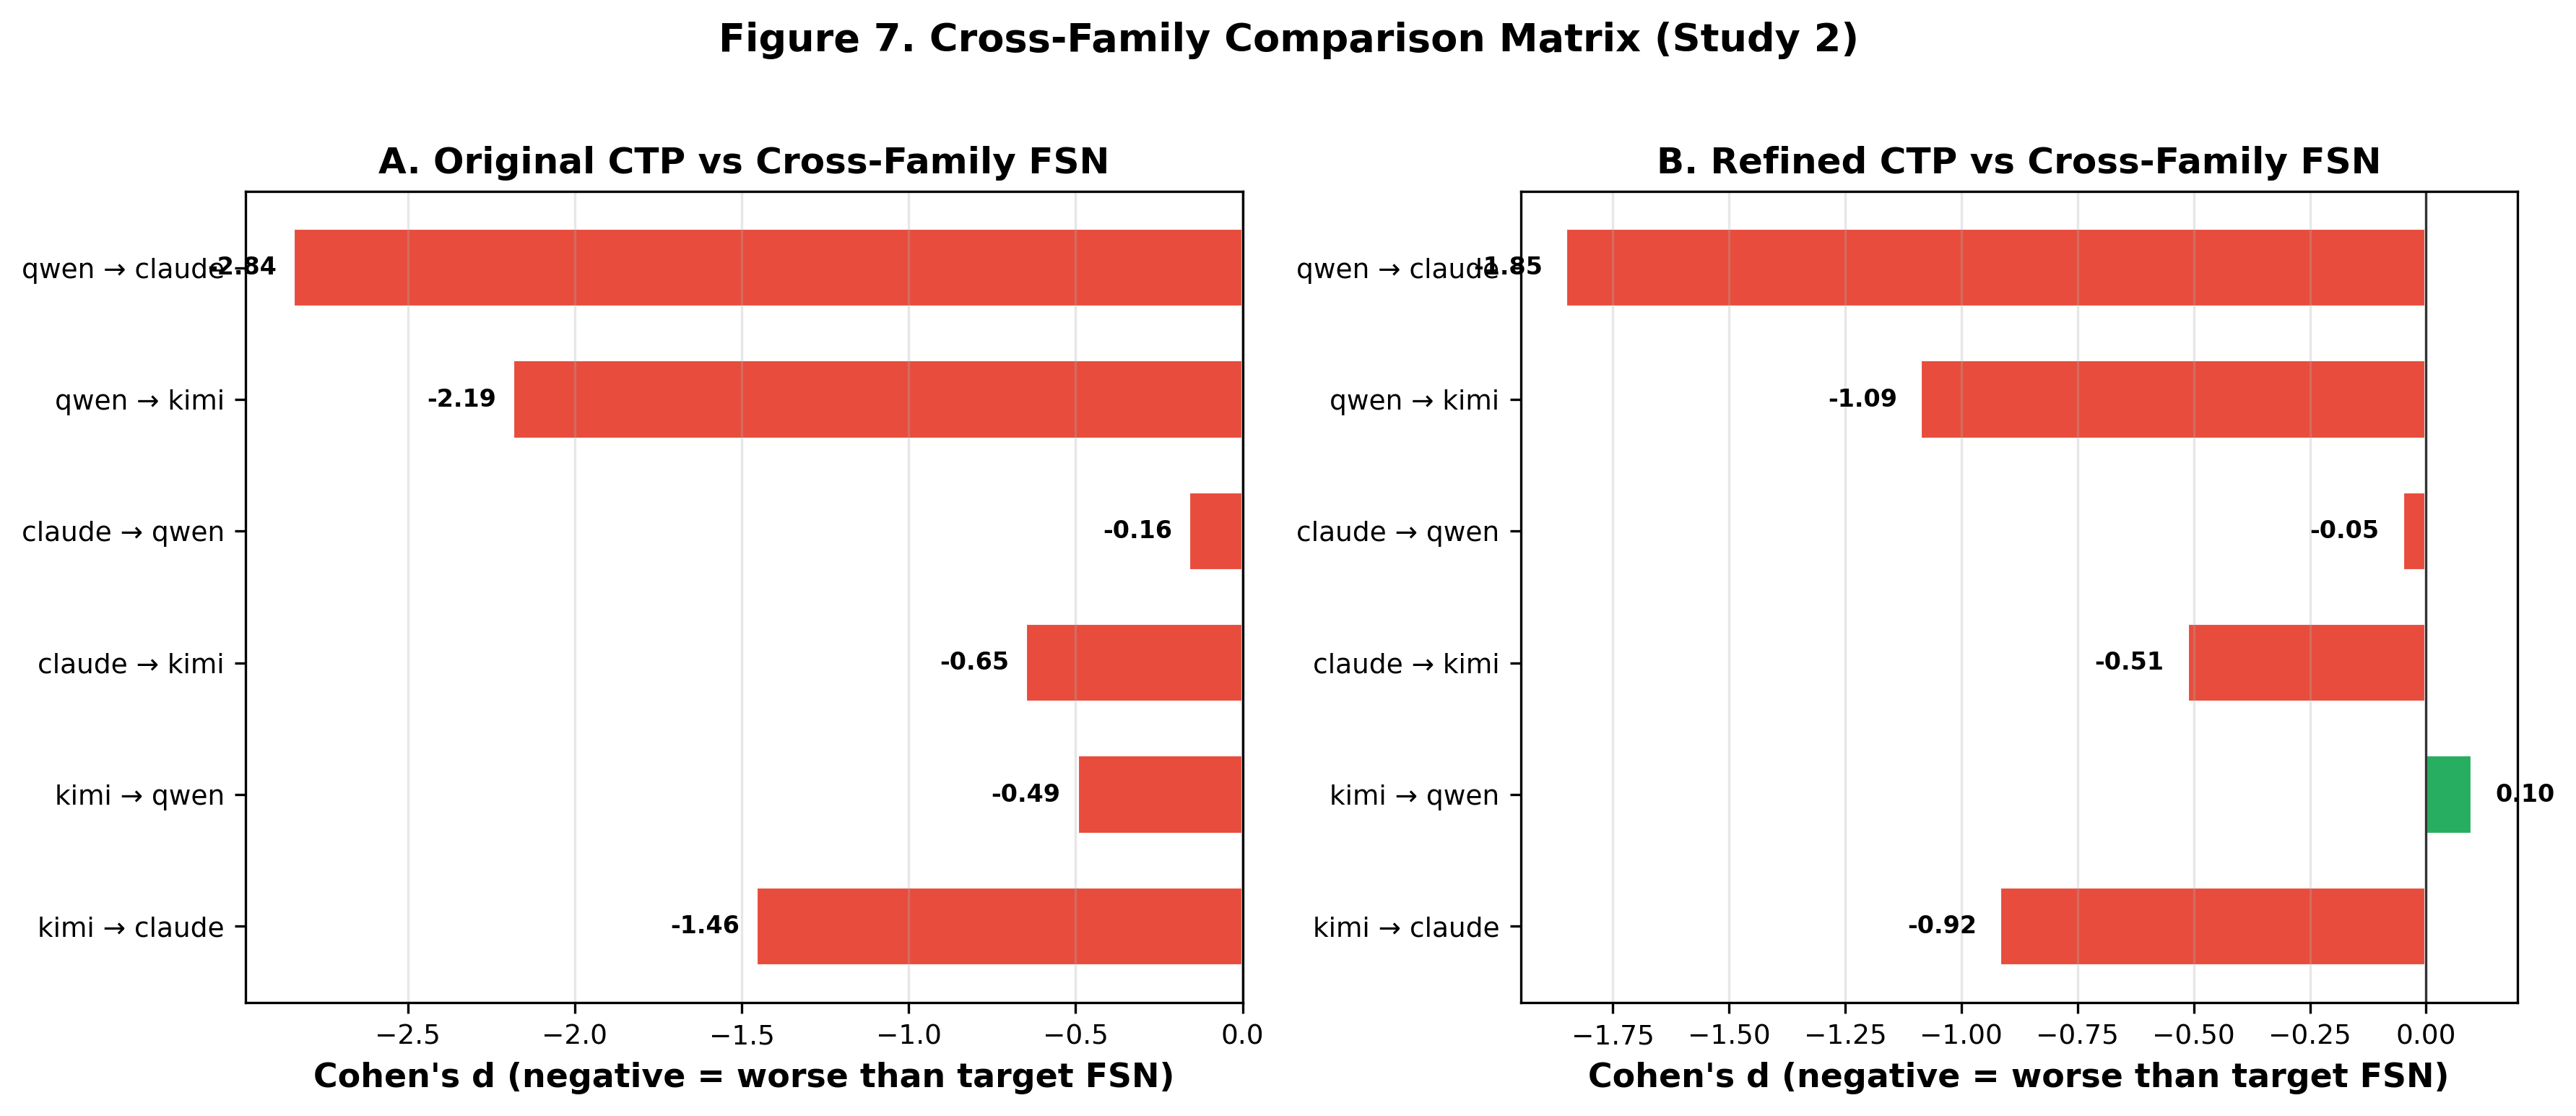
\includegraphics[width=\textwidth]{figures/fig7_cross_family_matrix.png}
  \caption{Cross-Family Comparison Matrix (Study~2).}
  \label{fig:cross-family}
\end{figure}

\subsection{Why Orchestration Buys Coverage but Not Density}\label{sec:mechanism}

Thirty triples (10 per family) are coded under a 13-code codebook. Pooled
Cohen's $\kappa = 0.824$ (93.1\% agreement), well above the 0.70 gate. Six of
the thirteen codes fall below 0.70 (\texttt{diagnostic\_reframe} 0.54,
\texttt{named\_concepts} 0.49, \texttt{assumption\_test} 0.56,
\texttt{structured\_report} 0.59, \texttt{external\_authority} 0.56,
\texttt{redundancy\_bloat} 0.65), a base-rate artifact: percentage agreement on
these codes ranges from 82\% to 98\%, but $\kappa$ is depressed by near-zero
prevalence. Conclusions on below-threshold codes are disclosed as medium
reliability.

Of the six codes whose prevalence changed between original and refined (kimi,
qwen), all six are \emph{structural scaffolding} codes:
\texttt{operational\_parameters}, \texttt{structured\_report},
\texttt{phased\_timeline}, \texttt{tables\_matrices},
\texttt{quantified\_targets}, \texttt{granular\_ops\_detail}. No insight code
(\texttt{diagnostic\_reframe}, \texttt{named\_concepts},
\texttt{assumption\_test}, \texttt{concise\_maxims}) moved. The convergence
metric shows refinement does not consistently move cheap outputs toward the
frontier on insight codes (kimi toward~4 / away~6; qwen 5/4; claude 0/2 ---
claude was already at ceiling).

The residual frontier edge is precisely located. The only $\kappa$-reliable
frontier-vs-refined difference $\ge 0.30$ is \texttt{concise\_maxims}: qwen
frontier 1.00 vs.\ refined 0.55 (gap~0.45). The medium-reliability
\texttt{redundancy\_bloat} code is 0.00 in every frontier sample and 0.65--0.95
in every refined sample. Claude's original answers are already at the codebook
ceiling ($\ge 0.90$ on 11 of 13 codes); the number of changed codes between
original and refined is zero --- a saturation mechanism that explains the 8\%
gap recovery in~\cref{sec:refinement}.

\begin{quote}
\textbf{Strategic Implication:} Orchestration is a coverage play --- it adds
structure, length, and completeness. The frontier's advantage is a density
play --- compressed insight with zero waste. Add-only refinement cannot
manufacture density, which explains why cheap teams approach but do not surpass
frontier quality.
\end{quote}

\begin{figure}[ht]
  \centering
  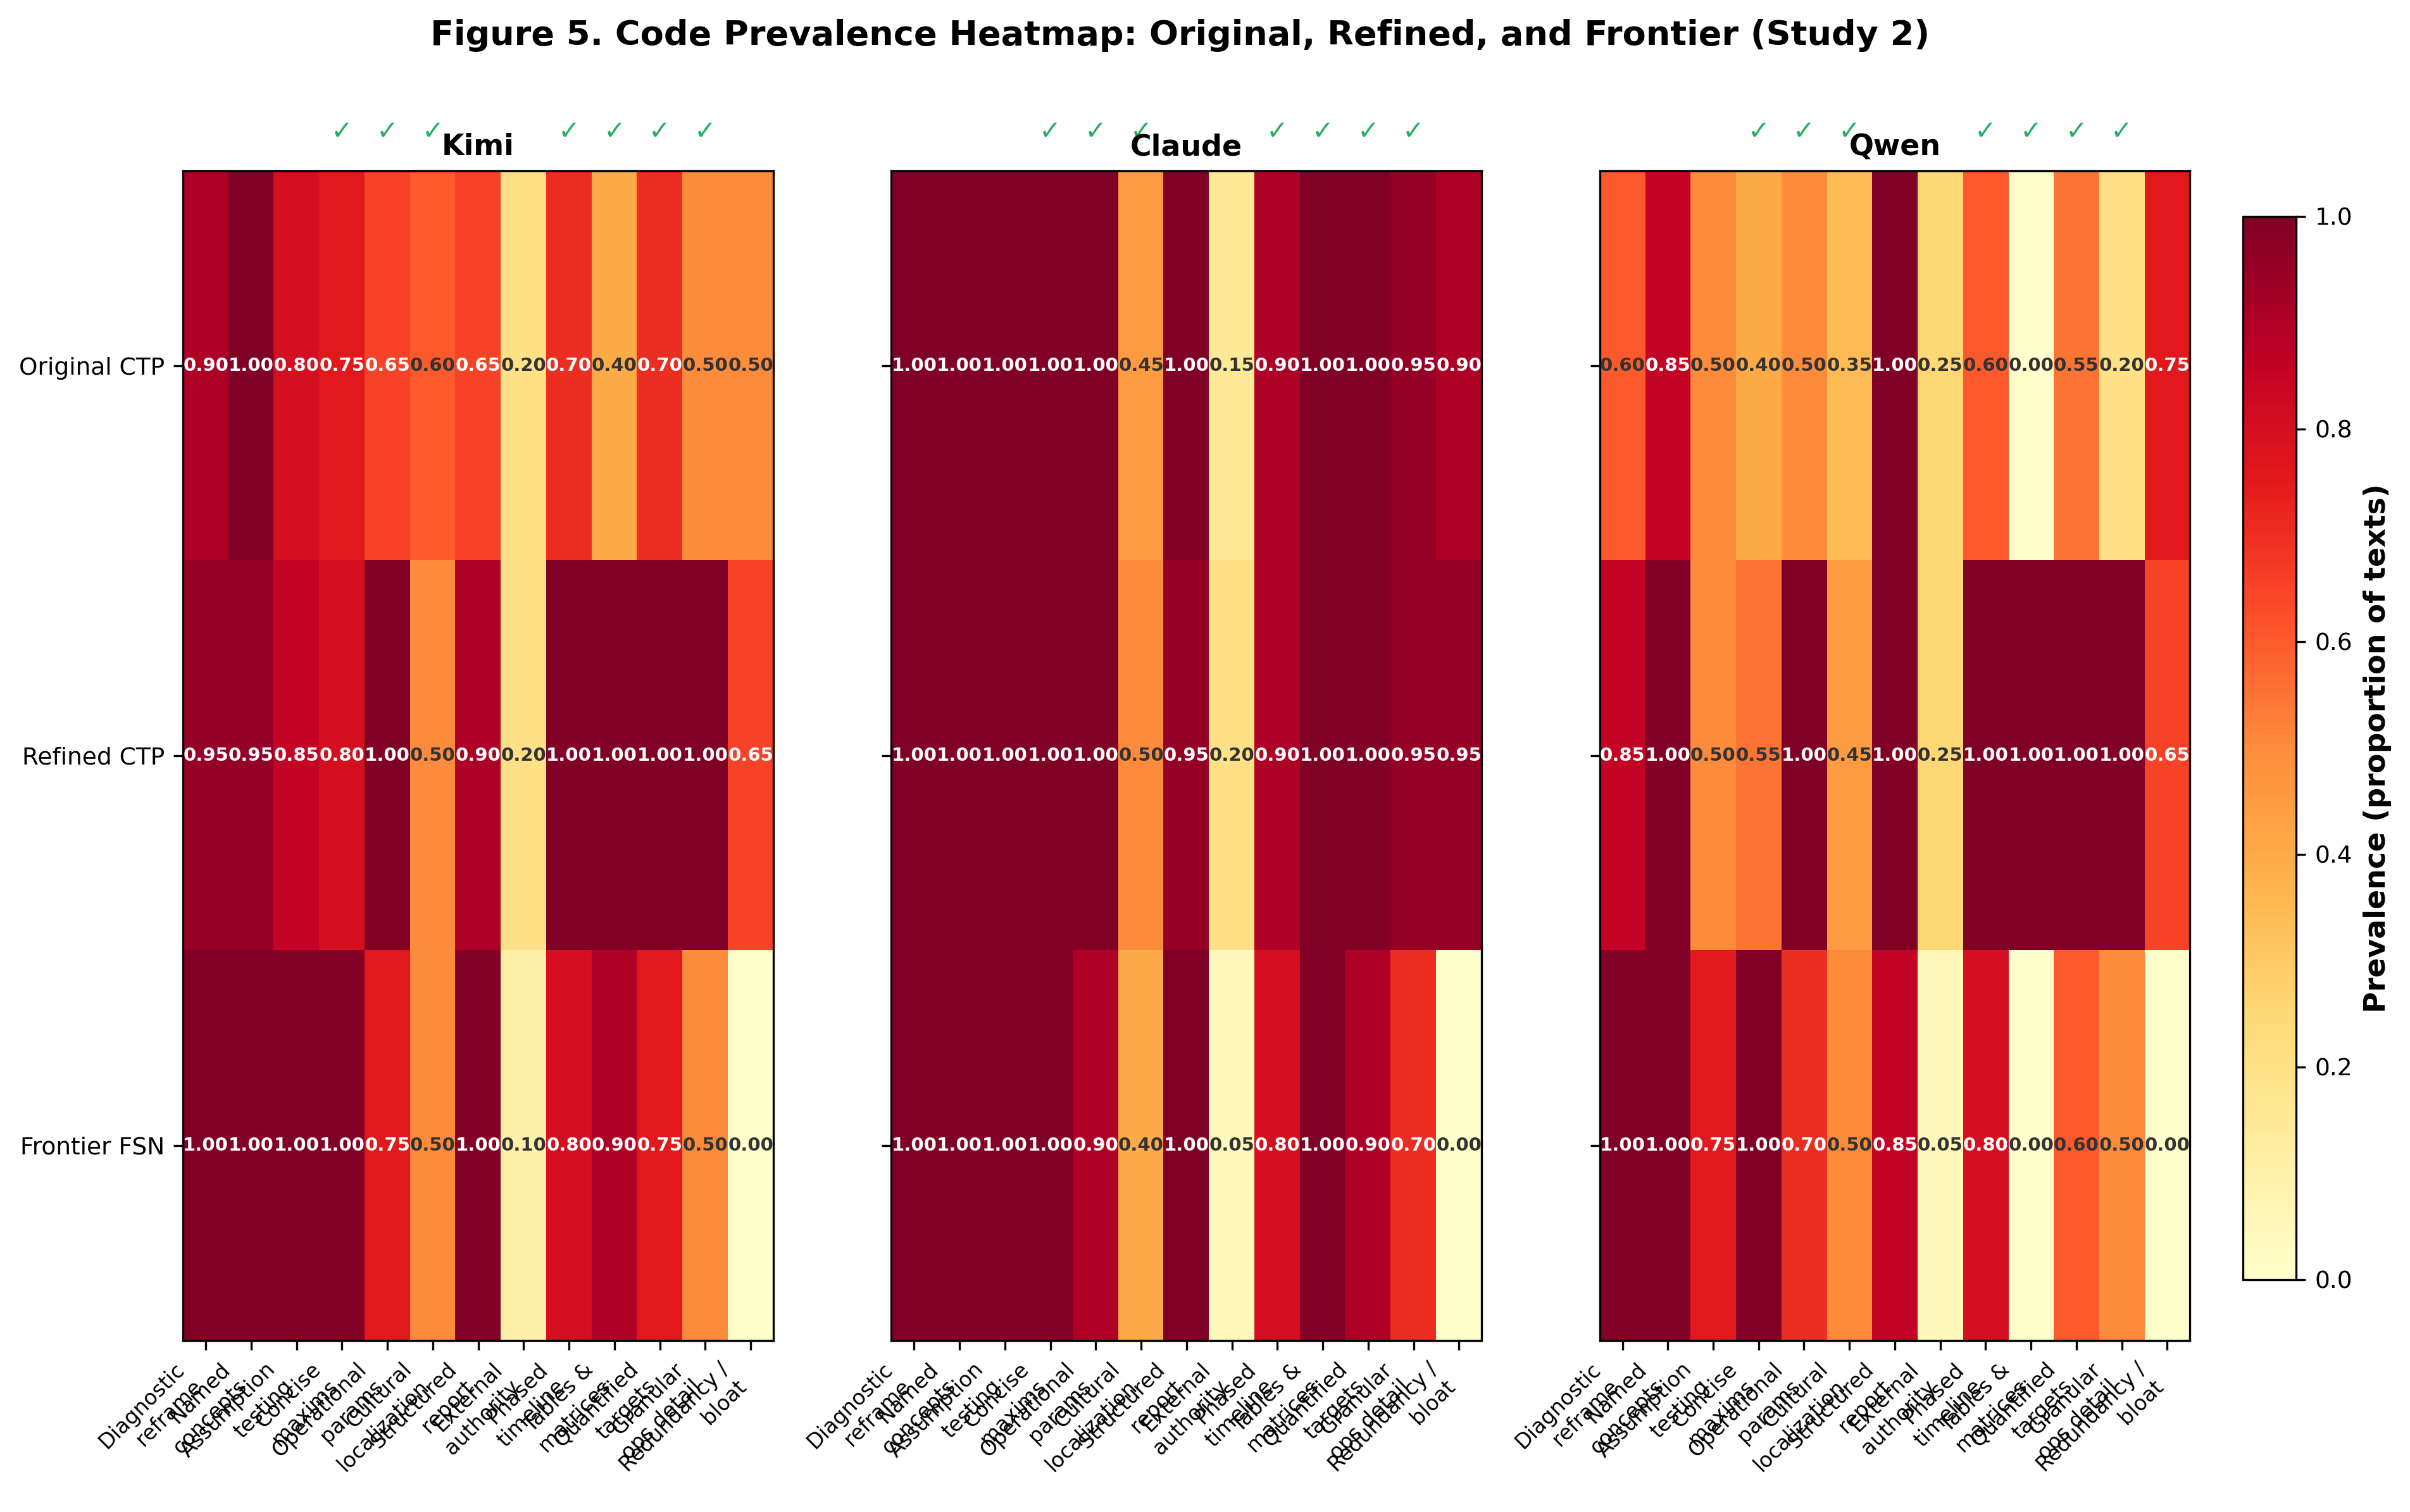
\includegraphics[width=\textwidth]{figures/fig5_code_heatmap.png}
  \caption{Code Prevalence Heatmap: Original, Refined, and Frontier (Study~2).}
  \label{fig:heatmap}
\end{figure}

\subsection{The Pareto Frontier: Optimal Configurations for Budget-Constrained
Firms}\label{sec:pareto}

The cost--quality map is shown in \cref{fig:cost-scatter}. At the primary
$\phiBlend = 0.50$, the cell means are:

\begin{table}[ht]
  \centering
  \caption{Cell summary statistics (primary analysis, $\phiBlend = 0.50$).}
  \label{tab:cell-summary}
  \begin{tabular}{@{}lrrrr@{}}
    \toprule
    \textbf{Cell} & \textbf{$n$} & \textbf{Cost (USD)} & \textbf{Quality} & \textbf{T-EGR} \\
    \midrule
    C-S-P & 285 & 0.0145 & 4.210 & 8.60 \\
    C-S-N & 285 & 0.0194 & 4.507 & 6.15 \\
    C-T-P & 285 & 0.0715 & 4.327 & 1.58 \\
    C-T-N & 285 & 0.0734 & 4.531 & 1.49 \\
    F-S-P & 190 & 0.0670 & 4.406 & 1.36 \\
    F-S-N & 190 & 0.0835 & 4.586 & 1.00 (base) \\
    F-T-N & 190 & 0.2951 & 4.610 & 0.27 \\
    F-T-P & 190 & 0.3044 & 4.370 & 0.27 \\
    \bottomrule
  \end{tabular}
\end{table}

\begin{figure}[ht]
  \centering
  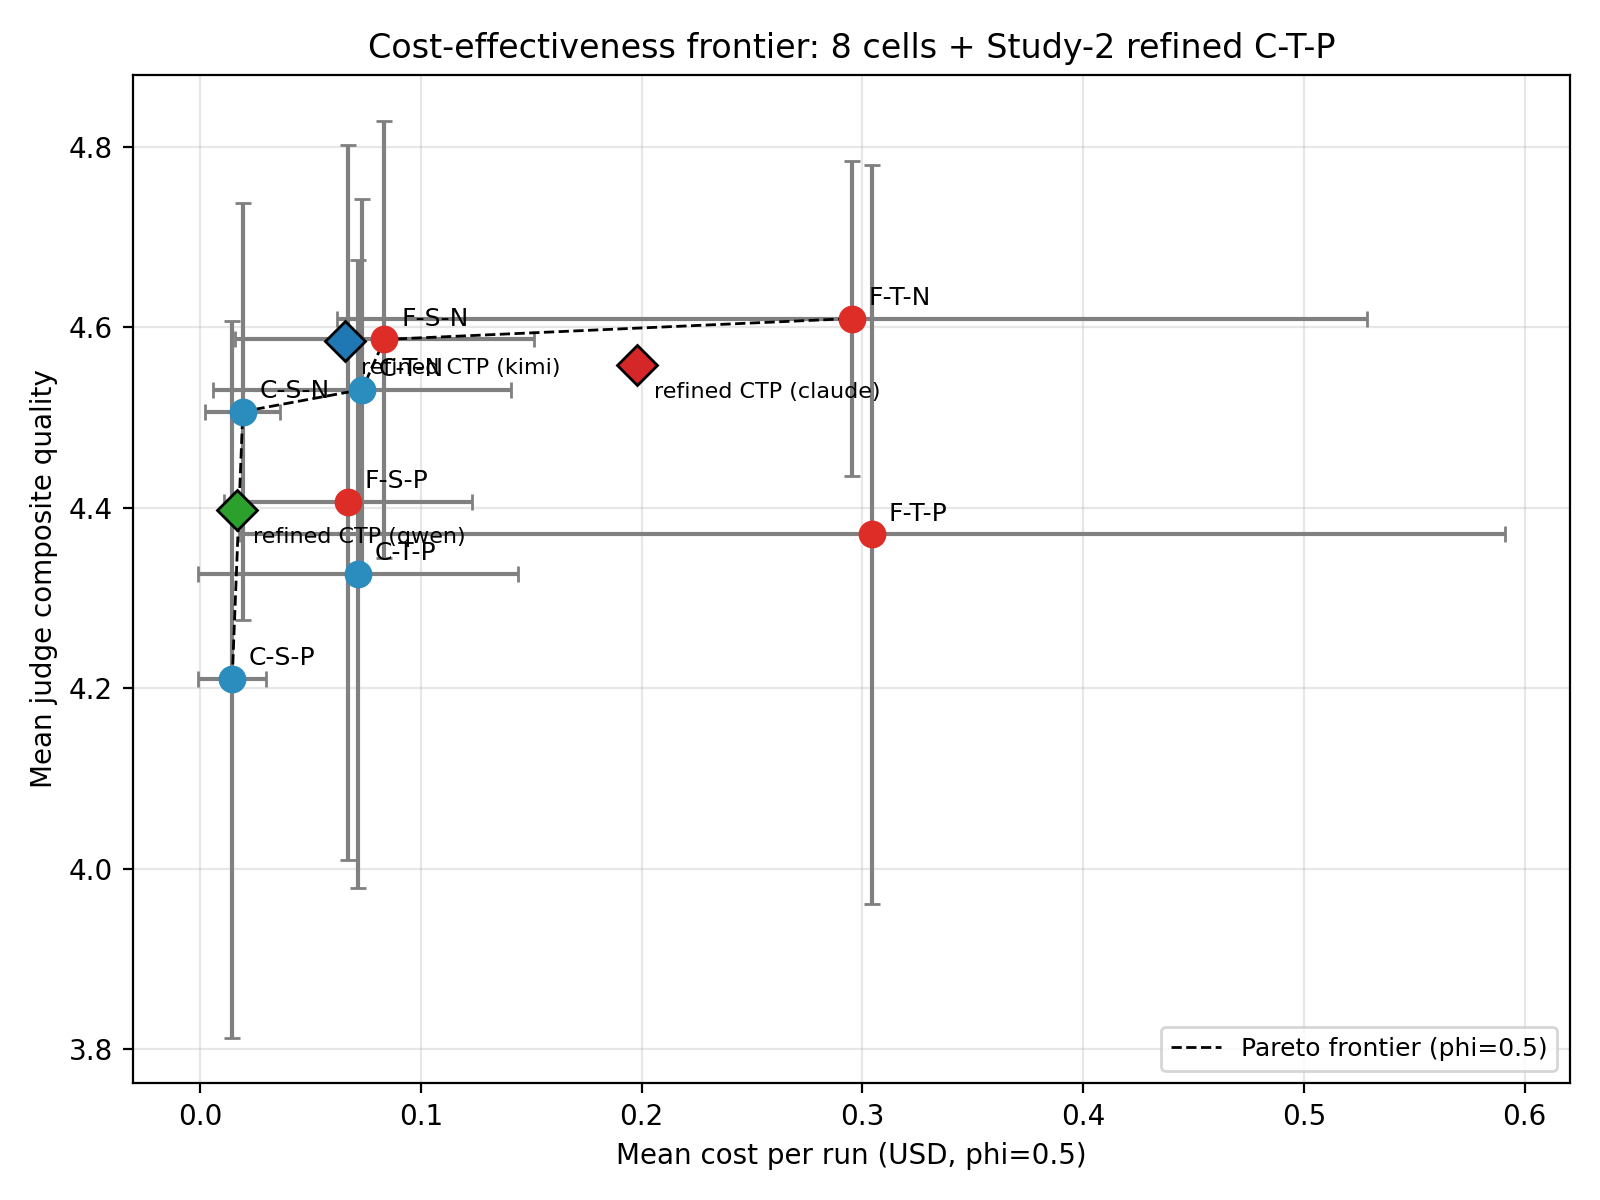
\includegraphics[width=\textwidth]{figures/fig3_cost_scatter.png}
  \caption{Cost-Effectiveness Frontier: 8 Cells + Study-2 Refined CTP.}
  \label{fig:cost-scatter}
\end{figure}

\begin{figure}[ht]
  \centering
  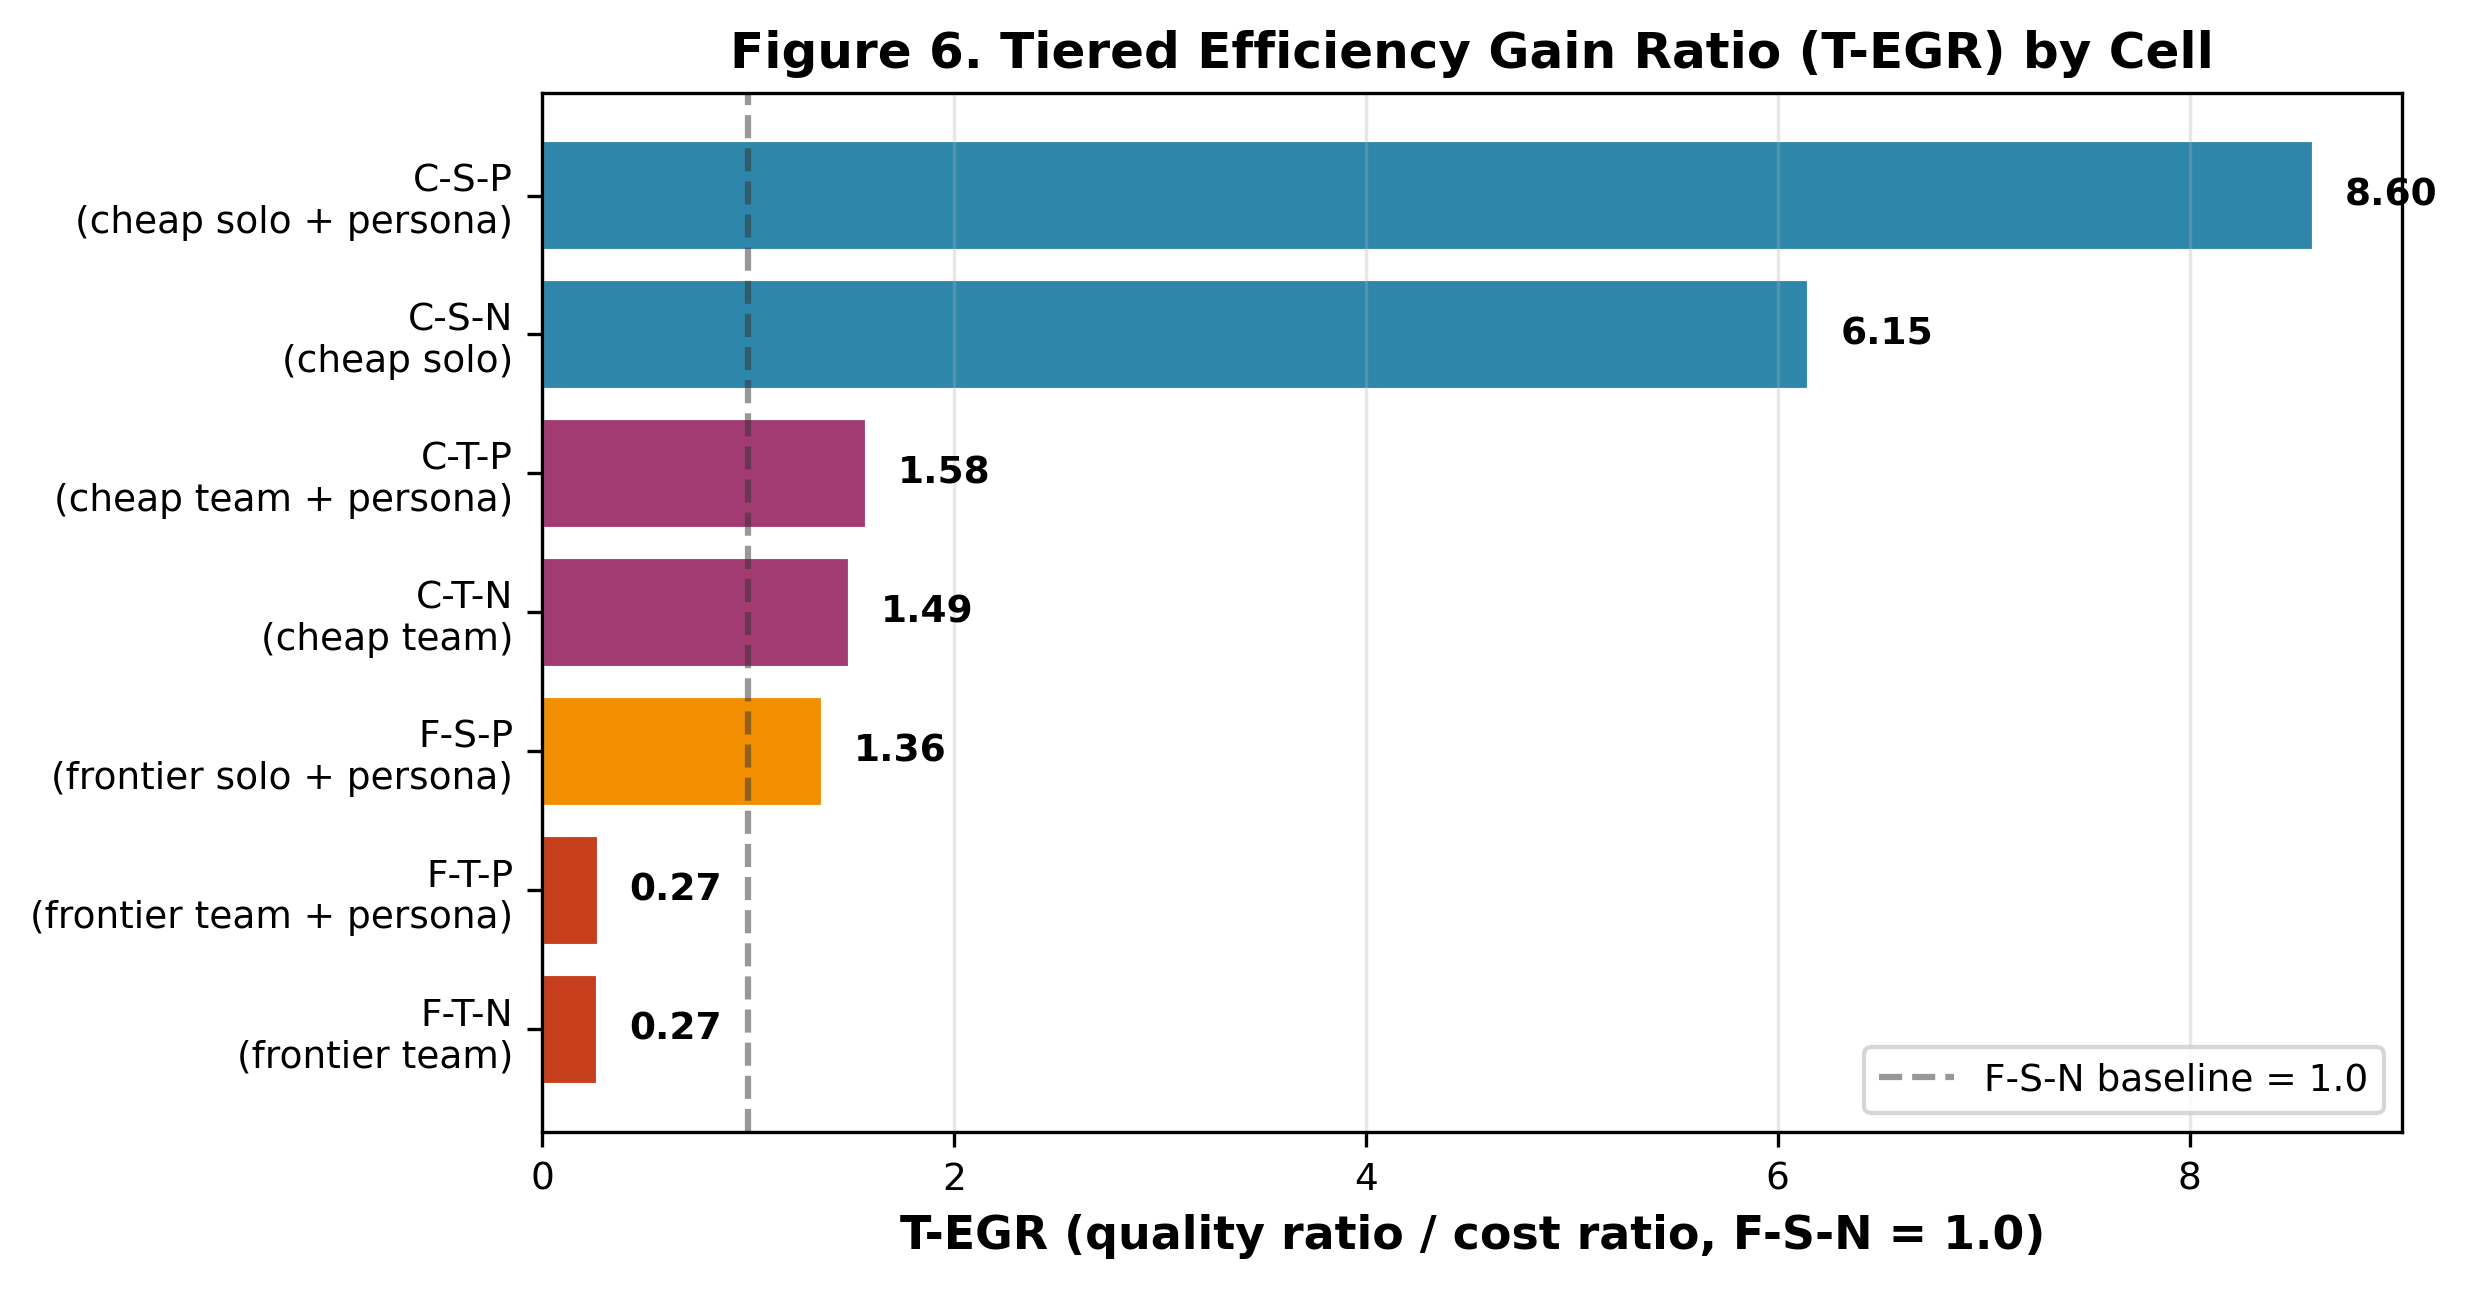
\includegraphics[width=\textwidth]{figures/fig6_tegr_bars.png}
  \caption{Tiered Efficiency Gain Ratio (T-EGR) by Cell.}
  \label{fig:tegr-bars}
\end{figure}

The Pareto frontier is \textbf{identical across all three $\phiBlend$}:
\{C-S-P, C-S-N, C-T-N, F-S-N, F-T-N\}. The dominated set \{C-T-P, F-S-P,
F-T-P\} contains every persona-loaded team cell --- the economic echo of the
\cref{sec:persona-penalty} persona penalty. Frontier membership is stable across
the sensitivity panel, satisfying the pre-registered claim rule.

\begin{figure}[ht]
  \centering
  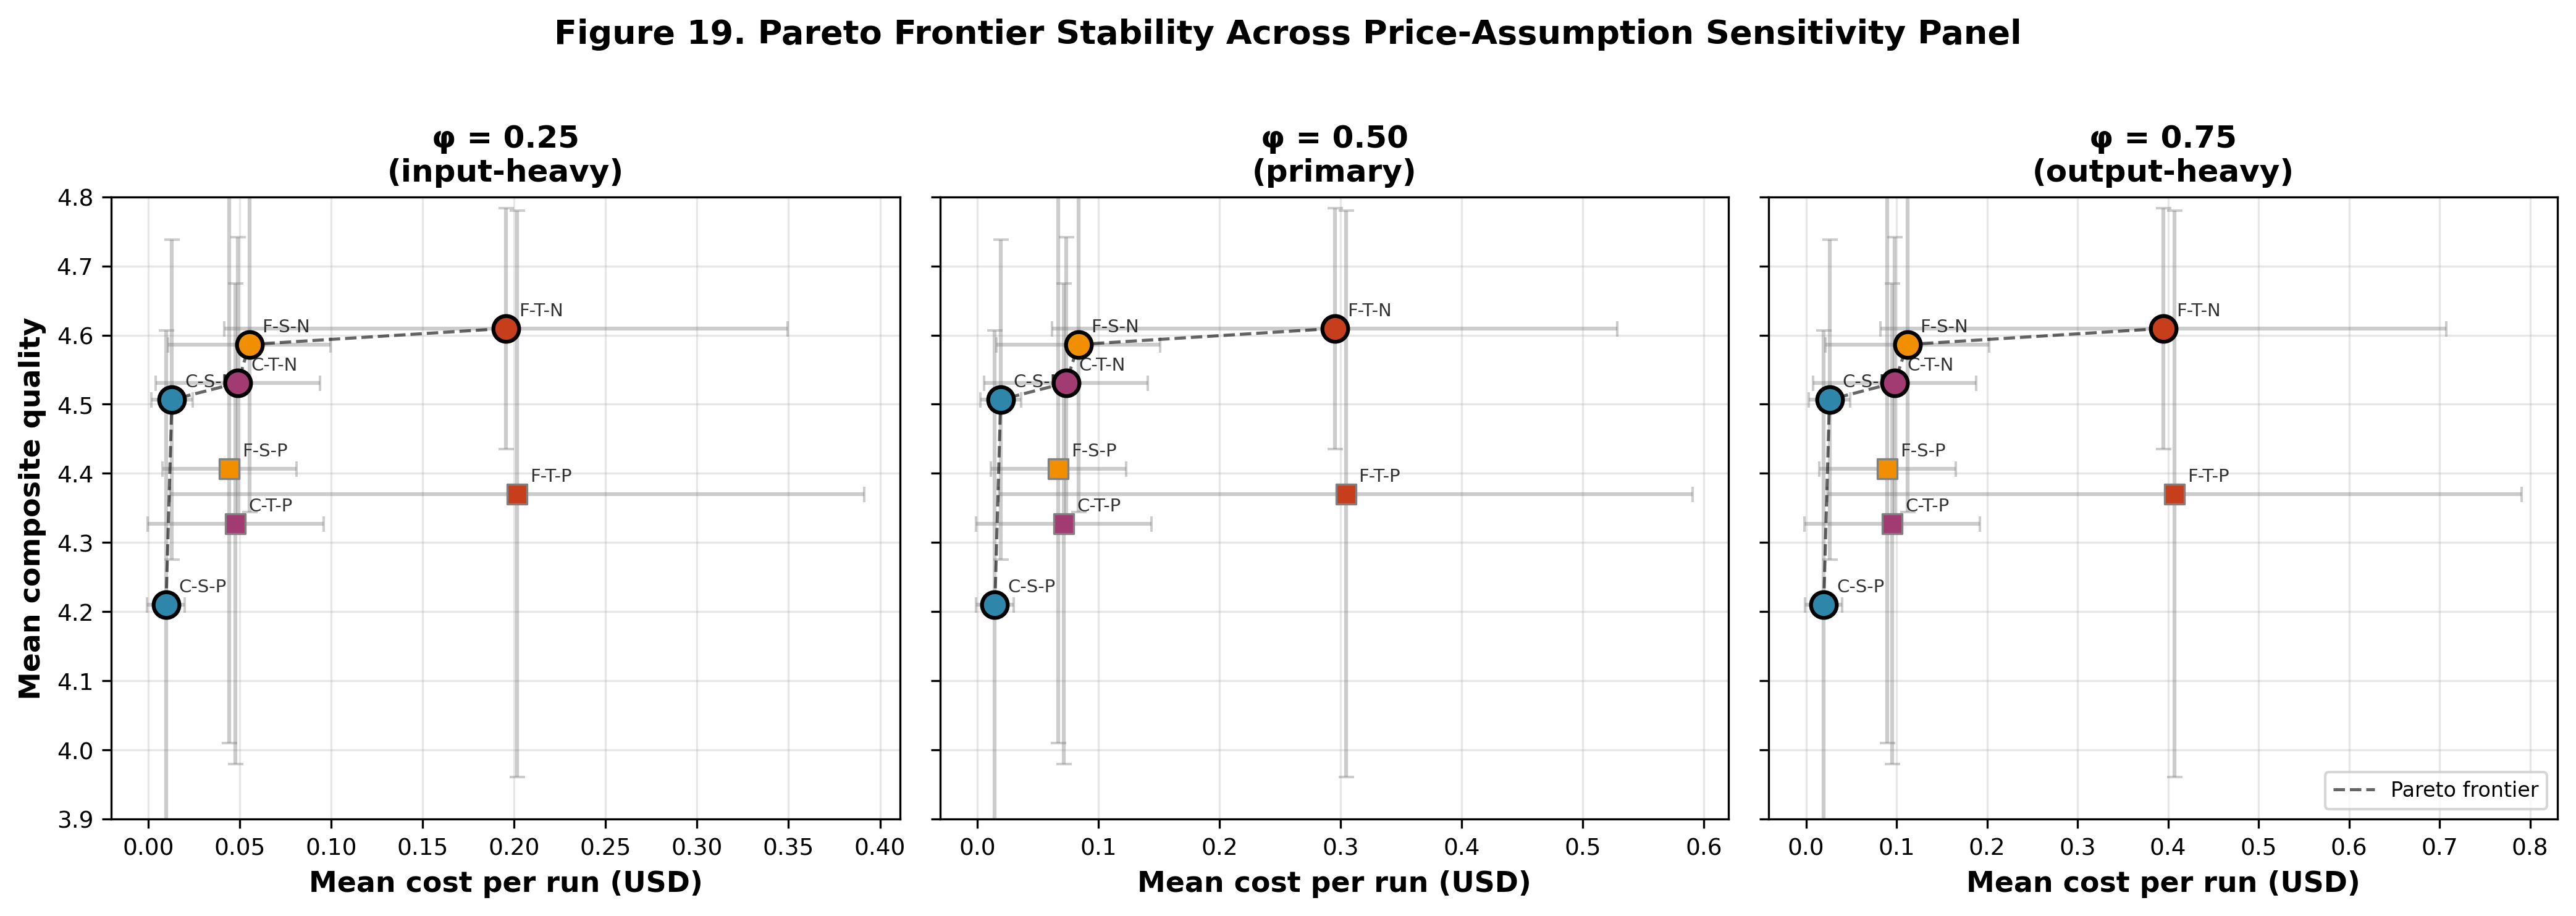
\includegraphics[width=\textwidth]{figures/fig19_phi_sensitivity.png}
  \caption{Pareto frontier stability across the price-assumption sensitivity
    panel. Left: $\phiBlend = 0.25$ (input-heavy blend). Center: $\phiBlend =
    0.50$ (primary analysis). Right: $\phiBlend = 0.75$ (output-heavy blend).
    The frontier set \{C-S-P, C-S-N, C-T-N, F-S-N, F-T-N\} is identical in all
    three panels, satisfying the pre-registered cross-$\phiBlend$ stability
    rule.}
  \label{fig:phi-sensitivity}
\end{figure}

ICER (vs.\ the cheapest cell, C-S-P): C-S-N is the best buy at +\$0.016 per
point of composite quality; F-T-P is the worst at +\$1.81 per point. The
refined kimi C-T-P point (not in the table) sits at \$0.0654 / quality~4.585 ---
absolute parity with pooled F-S-N (4.586) at 78\% of its cost, with the caveat
that the paired within-family comparison remains negative (disclosure
per~\cref{sec:refinement}).

\begin{quote}
\textbf{Strategic Implication:} The economically optimal strategy is to
substitute structure for tier at the cheap end (C-S-N: 98\% of frontier quality
at 23\% of the cost). The worst dollar in the experiment is spent on frontier
teams --- they cost 3.5$\times$ the frontier-solo price for negligible quality
gain.
\end{quote}

\subsection{Robustness: Do the Results Hold Across Model Families?}

The A2 battery supports the \cref{sec:interaction} decision.
Leave-one-family-out: $d$ ranges from $-0.143$ (drop kimi) to $-0.303$ (drop
gemini), sign stable in all five folds; no single family drives the
interaction. Leave-one-problem-out: $d$ ranges from $-0.212$ to $-0.247$ across
all 19 folds; no problem drives the interaction. Sensitivity power at the
smallest cell ($n = 190$) detects $d = 0.288$ at 80\% power; the observed $|d|
= 0.227$ is detected through the within-subjects contrast over all 1{,}900 runs
rather than per-cell power~(A2.7). Length adjustment on the $H_1$ contrast
yields $p = 0.63$ --- the interaction is not a length confound. The
random-effects meta-analysis over the five families~(A3.4) gives a pooled $d =
-0.270$ (CI $[-0.472, -0.069]$, $z = -2.64$, $p = 0.008$) with low-moderate
heterogeneity ($\tau^2 = 0.015$, $I^2 = 28.5\%$), confirming the interaction
generalizes.

Results are stable (mean absolute change of cell composite under the battery
$< 0.04$ across perturbations). The leave-one-out sensitivity (\cref{fig:loo})
and random-effects meta-analysis (\cref{fig:meta-analysis}) confirm that no
single family, problem, or outlier drives the result.

\begin{quote}
\textbf{Strategic Implication:} The findings are robust to judge, model family,
problem domain, and output-length variations. The interaction is small but
reliable and generalizes across the five leading LLM families --- a stable
result for firms making platform-agnostic investment decisions.
\end{quote}

\begin{figure}[ht]
  \centering
  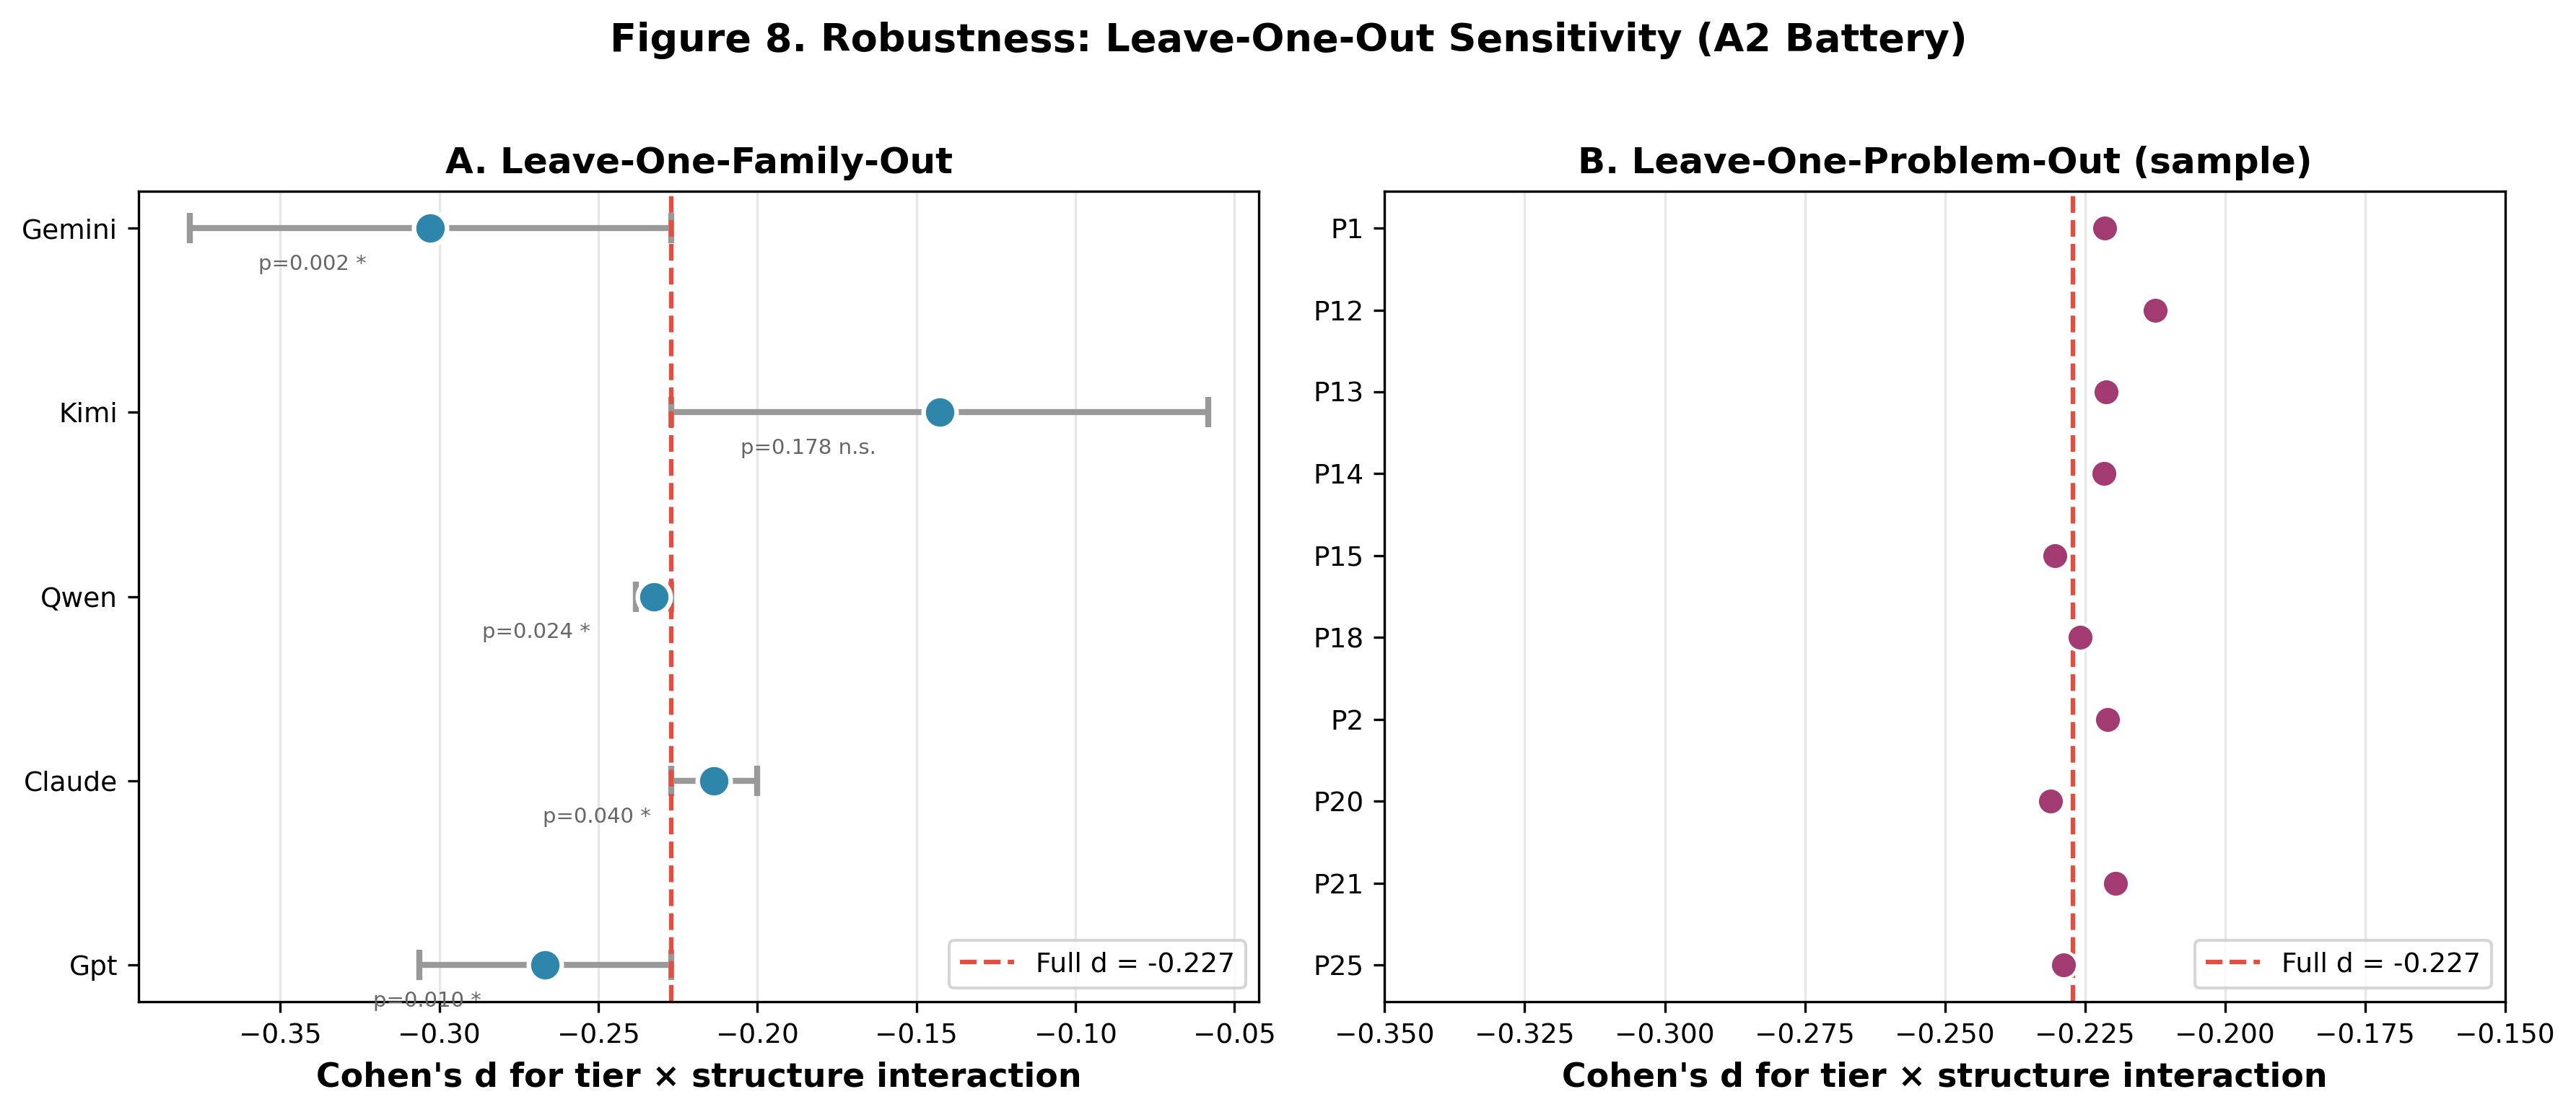
\includegraphics[width=\textwidth]{figures/fig8_robustness_loo.png}
  \caption{Robustness: Leave-One-Out Sensitivity (A2 Battery).}
  \label{fig:loo}
\end{figure}

\begin{figure}[ht]
  \centering
  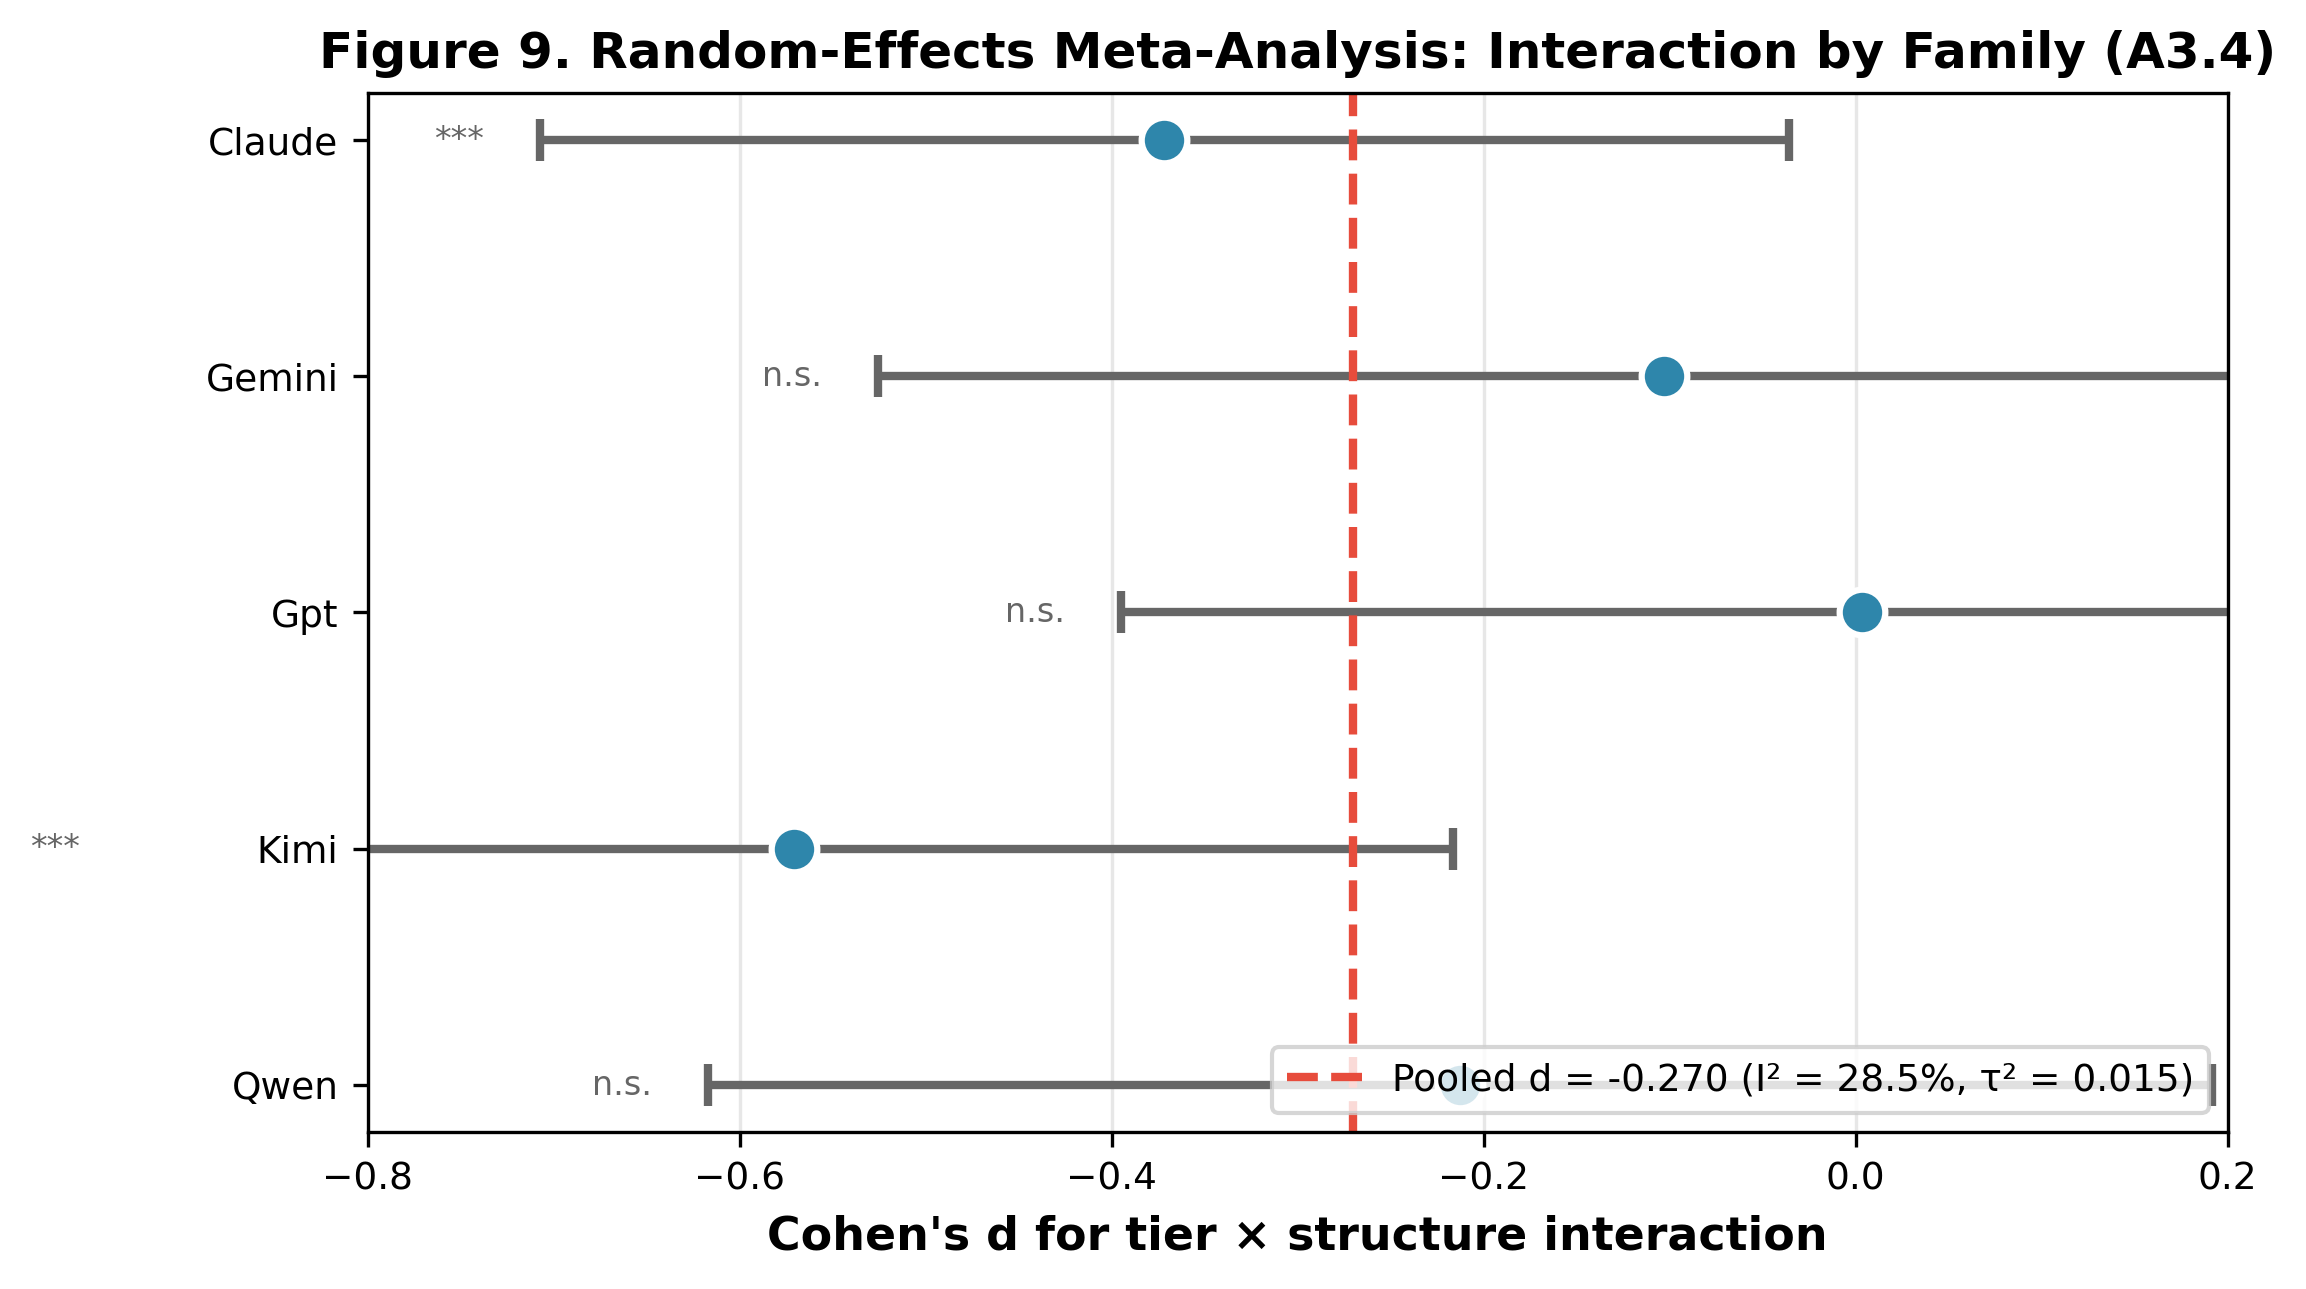
\includegraphics[width=\textwidth]{figures/fig9_meta_analysis_forest.png}
  \caption{Random-Effects Meta-Analysis: Interaction by Family.}
  \label{fig:meta-analysis}
\end{figure}

\subsection{Summary of Key Findings}

\begin{table}[ht]
  \centering
  \caption{Summary of key findings.}
  \label{tab:summary-findings}
  \begin{tabularx}{\textwidth}{@{}l l c@{}}
    \toprule
    \textbf{Finding} & \textbf{Evidence} & \textbf{Section} \\
    \midrule
    Team structure helps cheap more than frontier & $d = -0.227$ & \cref{sec:interaction} \\
    Frontier $>$ cheap overall & $d = +0.294$ & \cref{sec:interaction} \\
    Persona penalty on net & $d = -0.691$ & \cref{sec:interaction} \\
    Persona-loaded cells Pareto-dominated & cost--quality plane & \cref{sec:persona-penalty} \\
    CTP $<$ FSN in every family & paired comparisons & \cref{sec:frontier-gap} \\
    Refinement recovers 60--64\% of gap; G2 FAIL & $H_2$ tests & \cref{sec:refinement} \\
    Orchestration buys coverage; frontier wins on density & $\kappa = 0.824$; 13 codes & \cref{sec:mechanism} \\
    Pareto frontier stable across $\phiBlend$ & \{C-S-P, C-S-N, C-T-N, F-S-N, F-T-N\} & \cref{sec:pareto} \\
    \bottomrule
  \end{tabularx}
\end{table}

% ==================================================================
% 5  DISCUSSION
% ==================================================================
\section{Discussion}\label{sec:discussion}

\subsection{A Decision Framework for AI Investment}\label{sec:decision-framework}

The results support a contingency framework for AI investment rather than a
universal rule. For budget-constrained firms, \textbf{invest in cheap-team
pipelines for coverage-sensitive tasks} (timelines, matrices, quantified
targets): C-S-N achieves 98\% of frontier quality at 23\% of the cost
($\TEGR$~6.15) --- the highest-return configuration in the study. \textbf{Do not
orchestrate at the frontier tier}: frontier team cells spend 3.5$\times$ the
frontier-solo cost for +0.024 points of quality ($\TEGR$~0.27), making them the
worst dollar in the experiment. \textbf{Use a cheap refinement pass as a
risk-mitigation strategy} when absolute quality parity is the target: the
refined kimi point reaches parity at 78\% of F-S-N's cost, the cheapest route to
that milestone. \textbf{Avoid personas}: they increase cost while degrading
quality --- a value-destroying configuration.

\begin{figure}[ht]
  \centering
  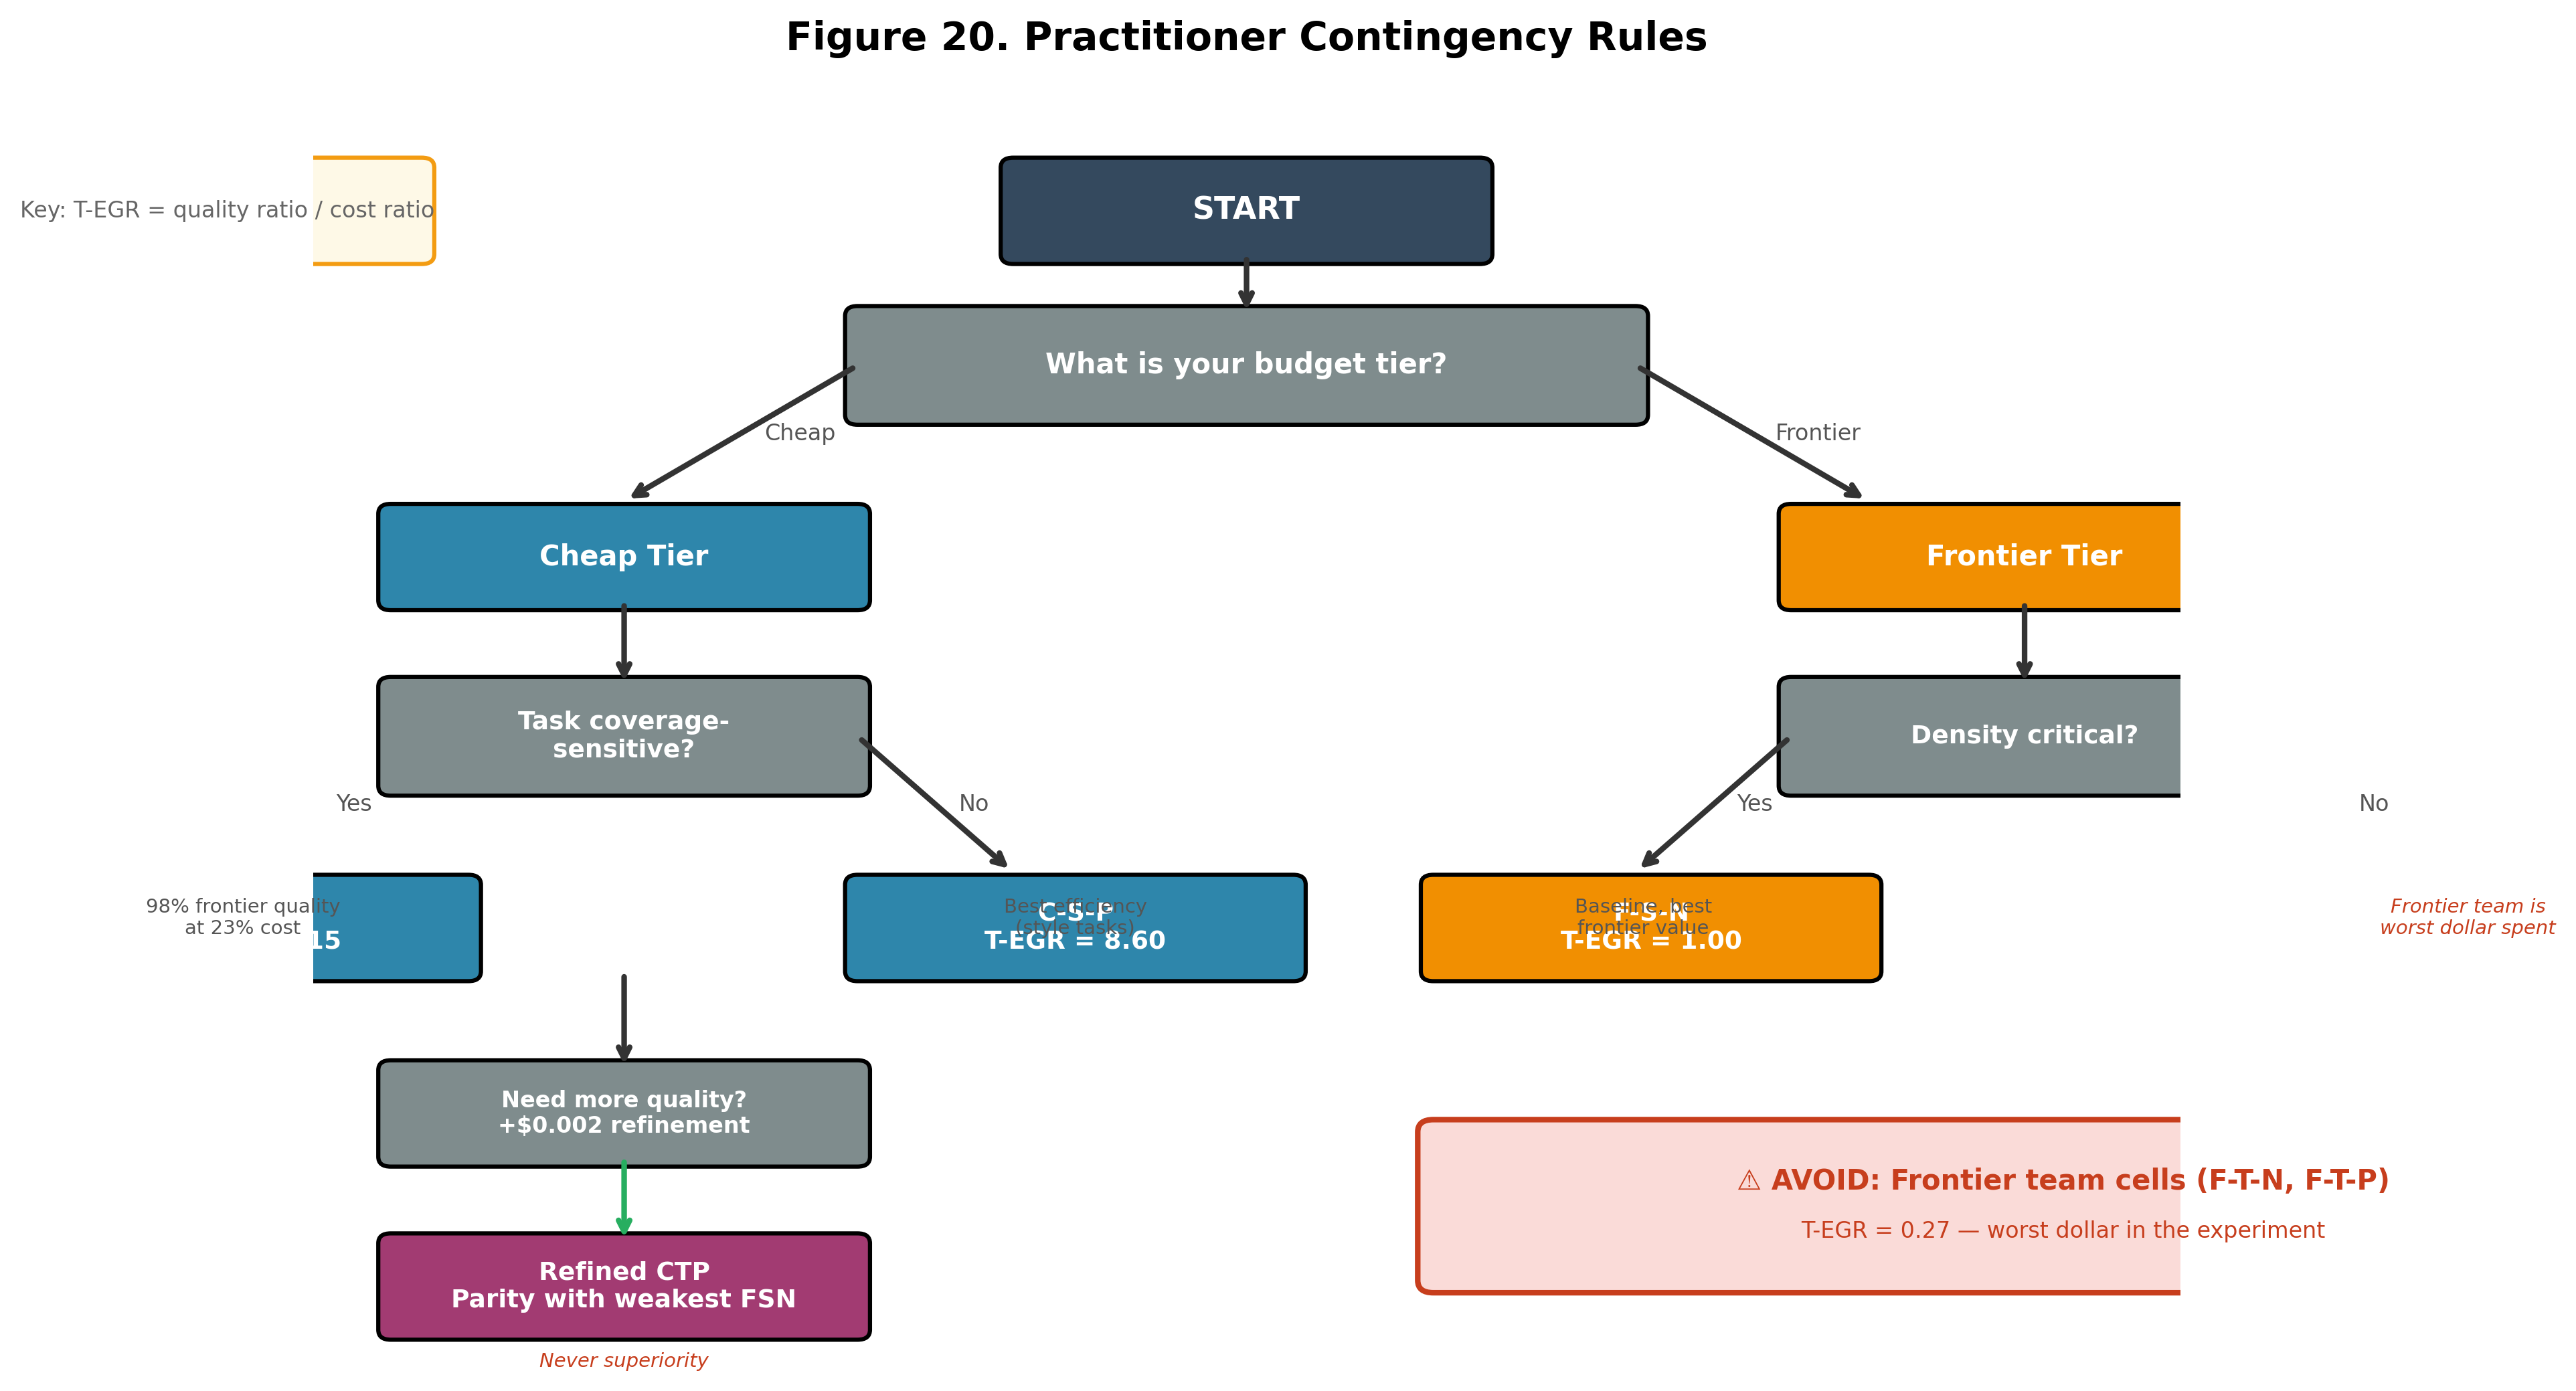
\includegraphics[width=\textwidth]{figures/fig20_contingency_rules.png}
  \caption{Practitioner contingency rules. Decision flowchart mapping budget
    tier and task type to the recommended orchestration cell, with expected
    T-EGR. Derived from the \cref{sec:decision-framework} contingency model.}
  \label{fig:contingency}
\end{figure}

\begin{table}[ht]
  \centering
  \caption{Managerial quick-reference: recommended configuration by task profile.}
  \label{tab:managerial}
  \begin{tabularx}{\textwidth}{@{}l l cc c l@{}}
    \toprule
    \textbf{Task profile} & \textbf{Cell} & \textbf{Quality} & \textbf{Cost} & \textbf{T-EGR} & \textbf{Override when\ldots} \\
    \midrule
    Coverage-heavy (plans, timelines, matrices)
      & C-S-N & 98\% & 23\% & 6.15
      & absolute quality non-negotiable $\to$ F-S-N \\
    Density-critical (exec briefs, strategic principles)
      & F-S-N & 100\% & 100\% & 1.00
      & budget tight $\to$ C-S-N at 98\% \\
    Budget-minimum, quality-adequate
      & C-S-P & 92\% & 17\% & 8.60
      & novelty needed, substance traded \\
    Refinement as risk mitigation
      & Refined C-T-P & $\sim$100\% & 78\% & ---
      & never achieves paired superiority \\
    \textbf{Avoid}
      & F-T-P, F-T-N & $\leq$100\% & 354\% & 0.27
      & worst dollar in the experiment \\
    \bottomrule
  \end{tabularx}
\end{table}

\subsection{The Density Ceiling: Why Additive Pipelines Hit a Wall}

The qualitative mechanism (\cref{sec:mechanism}) explains the pattern.
Orchestration is compositional --- add a critic, add a refiner, add a section,
add a table. Composition grows the answer but cannot compress it. The frontier's
residual advantage sits exactly where additive composition fails:
\texttt{concise\_maxims} (compressed, quotable strategic principles) and zero
\texttt{redundancy\_bloat}. These are the outputs of a single model that has
been selected or trained to produce dense prose. An add-only refiner, by design,
cannot delete the boilerplate the team structure produced. The falsifiable
prediction that follows is that a \emph{subtractive} refiner --- one permitted
to cut as well as add --- would narrow the density gap. This is the central
future-work experiment implied by our results.

\subsection{Contribution to the Business of AI Literature}

Our findings extend the author's prior lineage in two directions. The EGR metric
introduced in \citet{Hariri2026b} measured the cost performance of \emph{personas
in single models}; T-EGR extends it to teams and pipelines, preserving the ratio
form while re-basing on the frontier cell. The team-composition contingency
identified on verifiable tasks in \citet{Hariri2025b} reappears here on open-ended
tasks, but with the sign reversed for personas (harmful rather than neutral on
substance). The jagged-frontier finding of \citet{DellAcquaEtAl2023} is replicated
as a \emph{cell-level} result: cheap models inside the persona-free,
coverage-oriented region beat their cost-matched frontier alternatives; cheap
models pushed outside by persona-loading or by density demands fall below the
frontier.

The test-time-compute prediction of \citet{SnellEtAl2024} is partially confirmed:
more inference compute (team, refinement) improves the cheaper model, but only up
to a parity ceiling, and only when priced in dollars does the tradeoff reveal its
practitioner shape. Our contribution is the dollarization of the compute-optimal
curve on open-ended tasks where no verifier exists.

\subsection{Methodological Lessons for AI Deployment Research}

Two lessons carry beyond this study. First, preregistered negative superiority
results can be the spine of a paper, not its appendix. The G2 mechanical failure
in~\cref{sec:refinement} is as informative as any positive finding, and
preregistration is what made it reportable as a primary result rather than as a
null. Second, token-invariant costing --- storing tokens and re-pricing through a
frozen vector --- is reusable infrastructure for the field: every reported dollar
is reproducible by any reader who supplies an alternative price vector
\citep{Diewert1976, SandveEtAl2013}.


% ==================================================================
% 6  LIMITATIONS
% ==================================================================
\section{Limitations}\label{sec:limitations}

Four acknowledged limitations bound the claims. (1)~Evaluation is LLM-only; no
human panel was recruited. Our bias controls (blinding, order shuffle, disjoint
judge families, three prompt variants) follow the best current practice
\citep{ZhengEtAl2023, VergaEtAl2024} but do not substitute for human agreement
on a subset. (2)~The blended-$\phiBlend$ price assumption is a disclosed
limitation; we mitigate it with a pre-registered sensitivity panel and require
cross-$\phiBlend$ stability for any frontier-membership claim. (3)~The task
domain is English business strategy; generalization to code, scientific writing,
or non-English domains is an empirical question. (4)~Cross-family comparisons
(e.g.\ kimi vs.\ claude refinement rates) are descriptive and confounded with
family quality; only within-family comparisons support causal language. Two
further disclosures --- team intermediate outputs excluded from judged answers
(cost bias favorable to cheap teams) and a small truncation audit --- are stated
but not corrected.

A fifth limitation is practical: our costs are API-list prices, not
enterprise-negotiated rates. Firms with volume commitments or reserved-capacity
agreements may face different absolute prices, though the \emph{relative}
rankings (cheap tier $\approx$ 23\% of frontier) are preserved as long as the
price ratio between tiers remains in the 3--8$\times$ range observed across the
five families at the time of the experiment. Similarly, pipeline latency --- the
wall-clock time of three sequential API calls versus one --- is not priced here;
latency-sensitive applications may prefer frontier solo even when the dollar
cost favors the cheap pipeline.

% ==================================================================
% 7  FUTURE DIRECTIONS
% ==================================================================
\section{Future Directions}\label{sec:future}

Four experiments follow directly. First, a \textbf{subtractive refiner} study
that is permitted to cut as well as add: this isolates the density mechanism
identified in~\cref{sec:mechanism}. Second, a \textbf{human-panel replication}
on a subset of runs to bound LLM-judge bias in our specific design. Third, a
\textbf{second task domain} (code generation, scientific writing) to test
whether the coverage-vs-density mechanism generalizes beyond business strategy.
Fourth, \textbf{dynamic pricing integration}: the Qwen off-peak discount and
DeepSeek peak-surge windows suggest that time-of-day-aware orchestration may
shift the cost curve further; we registered the window but did not price the
study at realized paid prices.

% ==================================================================
% 8  CONCLUSION
% ==================================================================
\section{Conclusion}\label{sec:conclusion}

For organizations deploying LLMs for knowledge work, three investment rules
emerge from this 1{,}900-run experiment. \textbf{First}, at the cheap end,
structure substitutes for model tier: a three-step pipeline on a cheap model
delivers 98\% of frontier quality at 23\% of the cost ($\TEGR$~6.15) --- the
highest-return configuration tested. \textbf{Second}, at the frontier end, team
orchestration destroys value: it costs 3.5$\times$ the frontier-solo price for
negligible quality gain ($\TEGR$~0.27). \textbf{Third}, a cheap refinement pass
(\$0.002) recovers most of the frontier gap but never beats it --- a
bounded-improvement result that makes it a viable risk-mitigation strategy, not
a replacement strategy. The residual frontier advantage is density (compressed
insight, zero waste), not coverage --- a capability gap that add-only pipelines
cannot bridge. Personas are value-destroying: they increase cost while degrading
quality. The governing principle is contingency, not universality: match the
right pipeline architecture to the right model tier for the right task, and
invest in refinement before investing in a frontier team.

The broader implication is a build-versus-buy framework for AI capability.
Frontier models are \emph{bought} --- a fixed per-call cost for a given quality
level. Orchestration pipelines are \emph{built} --- an upfront architectural
investment that lowers marginal cost per call. Our results show that the build
path pays off when (a)~the task is coverage-sensitive, (b)~the quality bar is
``good enough'' rather than ``best available,'' and (c)~the firm can absorb the
engineering cost of maintaining a multi-step pipeline. When density is the
binding constraint --- when the output must compress insight into minimal prose
--- the buy path (frontier solo) remains optimal. The contingency is not a
limitation of the study; it is the finding.

For the field, the contribution is a dollarized, pre-registered, cost-matched
empirical test of the substitution claim that sits at the heart of the
multi-agent AI industry. The claim is partially true: structure does substitute
for tier, but only up to a ceiling set by density. That ceiling, and the
contingency rules that surround it, are the paper's contribution to the business
of~AI.

% ==================================================================
% REFERENCES
% ==================================================================
\begin{thebibliography}{99}

\bibitem[Abers and Lakens(2018)]{AlbersLakens2018}
Albers, C., \& Lakens, D. (2018).
When power analyses based on pilot data are biased: Inaccurate effect size
  estimators and follow-up bias.
\textit{Journal of Experimental Social Psychology}, \textit{74}, 187--195.
\href{https://doi.org/10.1016/j.jesp.2017.09.004}{doi:10.1016/j.jesp.2017.09.004}

\bibitem[Brynjolfsson et~al.(2023)]{BrynjolfssonLiRaymond2023}
Brynjolfsson, E., Li, D., \& Raymond, L.~R. (2023).
\textit{Generative AI at Work} (NBER Working Paper No.~31161).
\href{https://doi.org/10.3386/w31161}{doi:10.3386/w31161}

\bibitem[Cohen(1960)]{Cohen1960}
Cohen, J. (1960).
A coefficient of agreement for nominal scales.
\textit{Educational and Psychological Measurement}, \textit{20}(1), 37--46.
\href{https://doi.org/10.1177/001316446002000104}{doi:10.1177/001316446002000104}

\bibitem[Dell'Acqua et~al.(2023)]{DellAcquaEtAl2023}
Dell'Acqua, F., McFowland~III, E., Mollick, E.~R., Lifshitz-Assaf, H.,
  Kellogg, K., Rajendran, S., Krayer, L., Candelon, F., \& Lakhani, K.~R.
  (2023).
\textit{Navigating the jagged technological frontier: Field experimental
  evidence of the effects of AI on knowledge worker productivity and quality}
  (HBS Working Paper No.~24-013).
\href{https://doi.org/10.2139/ssrn.4573321}{doi:10.2139/ssrn.4573321}

\bibitem[Diewert(1976)]{Diewert1976}
Diewert, W.~E. (1976).
Exact and superlative index numbers.
\textit{Journal of Econometrics}, \textit{4}(2), 115--145.
\href{https://doi.org/10.1016/0304-4076(76)90009-9}{doi:10.1016/0304-4076(76)90009-9}

\bibitem[Hariri(2025a)]{Hariri2025a}
Hariri, Y. (2025a).
\textit{LLM-Creativity} [dataset and paper]. Zenodo.
\href{https://doi.org/10.5281/zenodo.17407392}{doi:10.5281/zenodo.17407392}

\bibitem[Hariri(2025b)]{Hariri2025b}
Hariri, Y. (2025b).
\textit{LLM Team Composition Paradox} [dataset and paper]. Zenodo.
\href{https://doi.org/10.5281/zenodo.17490945}{doi:10.5281/zenodo.17490945}

\bibitem[Hariri(2026b)]{Hariri2026b}
Hariri, Y. (2026b).
\textit{Doing More with Less: How Cultural Personas Bridge the Cost--Performance
  Gap in LLMs}. Zenodo.
\href{https://doi.org/10.5281/zenodo.19533619}{doi:10.5281/zenodo.19533619}

\bibitem[Lakens(2013)]{Lakens2013}
Lakens, D. (2013).
Calculating and reporting effect sizes to facilitate cumulative science: A
  practical primer for $t$-tests and ANOVAs.
\textit{Frontiers in Psychology}, \textit{4}, 863.
\href{https://doi.org/10.3389/fpsyg.2013.00863}{doi:10.3389/fpsyg.2013.00863}

\bibitem[Liang et~al.(2024)]{LiangEtAl2024}
Liang, T., He, Z., Jiao, W., Wang, X., Wang, Y., Wang, R., Yang, Y., Shi, S.,
  \& Tu, Z. (2024).
Encouraging divergent thinking in large language models through multi-agent
  debate.
In \textit{Proceedings of the 2024 Conference on Empirical Methods in Natural
  Language Processing} (pp.~17889--17904).
\href{https://doi.org/10.18653/v1/2024.emnlp-main.992}{doi:10.18653/v1/2024.emnlp-main.992}

\bibitem[Nosek et~al.(2018)]{NosekEtAl2018}
Nosek, B.~A., Ebersole, C.~R., DeHaven, A.~C., \& Mellor, D.~T. (2018).
The preregistration revolution.
\textit{PNAS}, \textit{115}(11), 2600--2606.
\href{https://doi.org/10.1073/pnas.1708274114}{doi:10.1073/pnas.1708274114}

\bibitem[Noy and Zhang(2023)]{NoyZhang2023}
Noy, S., \& Zhang, W. (2023).
Experimental evidence on the productivity effects of generative artificial
  intelligence.
\textit{Science}, \textit{381}(6654), 187--192.
\href{https://doi.org/10.1126/science.adh2586}{doi:10.1126/science.adh2586}

\bibitem[Sandve et~al.(2013)]{SandveEtAl2013}
Sandve, G.~K., Nekrutenko, A., Taylor, J., \& Hovig, E. (2013).
Ten simple rules for reproducible computational research.
\textit{PLoS Computational Biology}, \textit{9}(10), e1003285.
\href{https://doi.org/10.1371/journal.pcbi.1003285}{doi:10.1371/journal.pcbi.1003285}

\bibitem[Shinn et~al.(2023)]{ShinnEtAl2023}
Shinn, N., Cassano, F., Berman, E., Gopinath, A., Narasimhan, K., \& Yao, S.
  (2023).
Reflexion: Language agents with verbal reinforcement learning.
In \textit{Advances in Neural Information Processing Systems 36 (NeurIPS 2023)},
  pp.~8634--8652.

\bibitem[Snell et~al.(2024)]{SnellEtAl2024}
Snell, C., Lee, J., Xu, K., \& Kumar, A. (2024).
Scaling LLM test-time compute optimally can be more effective than scaling model
  parameters.
arXiv:2408.03314.
\href{https://doi.org/10.48550/arXiv.2408.03314}{doi:10.48550/arXiv.2408.03314}

\bibitem[Steegen et~al.(2016)]{SteegenEtAl2016}
Steegen, S., Tuerlinckx, F., Gelman, A., \& Vanpaemel, W. (2016).
Increasing transparency through a multiverse analysis.
\textit{Perspectives on Psychological Science}, \textit{11}(5), 702--712.
\href{https://doi.org/10.1177/1745691616658637}{doi:10.1177/1745691616658637}

\bibitem[Tomlinson et~al.(2024)]{TomlinsonEtAl2024}
Tomlinson, B., Black, R.~W., Patterson, D.~J., \& Torrance, A.~W. (2024).
The carbon emissions of writing and illustrating are lower for AI than for
  humans.
\textit{Scientific Reports}, \textit{14}, 3732.
\href{https://doi.org/10.1038/s41598-024-54271-x}{doi:10.1038/s41598-024-54271-x}

\bibitem[Verga et~al.(2024)]{VergaEtAl2024}
Verga, P., Hofst\"atter, S., Althammer, S., Su, Y., Piktus, A.,
  Arkhangorodsky, A., Xu, M., White, N., \& Lewis, P. (2024).
Replacing judges with juries: Evaluating LLM generations with a panel of diverse
  models.
arXiv:2404.18796.
\href{https://doi.org/10.48550/arXiv.2404.18796}{doi:10.48550/arXiv.2404.18796}

\bibitem[Wang et~al.(2023)]{WangEtAl2023}
Wang, X., Wei, J., Schuurmans, D., Le, Q., Chi, E., Narang, S., Chowdhery, A.,
  \& Zhou, D. (2023).
Self-consistency improves chain of thought reasoning in language models.
In \textit{Proceedings of the Eleventh International Conference on Learning
  Representations} (ICLR 2023).

\bibitem[Wei et~al.(2022)]{WeiEtAl2022}
Wei, J., Wang, X., Schuurmans, D., Bosma, M., Ichter, B., Xia, F., Chi, E.,
  Le, Q., \& Zhou, D. (2022).
Chain-of-thought prompting elicits reasoning in large language models.
In \textit{Advances in Neural Information Processing Systems 35 (NeurIPS 2022)},
  pp.~24824--24837.

\bibitem[Yao et~al.(2023)]{YaoEtAl2023}
Yao, S., Yu, D., Zhao, J., Shafran, I., Griffiths, T.~L., Cao, Y., \&
  Narasimhan, K. (2023).
Tree of thoughts: Deliberate problem solving with large language models.
In \textit{Advances in Neural Information Processing Systems 36 (NeurIPS 2023)}.

\bibitem[Zheng et~al.(2023)]{ZhengEtAl2023}
Zheng, L., Chiang, W.-L., Sheng, Y., Zhuang, S., Wu, Z., Zhuang, Y., Lin, Z.,
  Li, Z., Li, D., Xing, E.~P., Zhang, H., Gonzalez, J.~E., \& Stoica, I.
  (2023).
Judging LLM-as-a-judge with MT-Bench and Chatbot Arena.
In \textit{Advances in Neural Information Processing Systems 36 (NeurIPS 2023)},
  Datasets and Benchmarks Track.

\end{thebibliography}

\end{document}
